\documentclass{classes/fiboReport}

\begin{document}

\Modifydate{21/04/2018}
\subject{FRA501 Principles of Model-based Design in Robotics}
\title{Quadrotor Dynamic Modelling}
\subtitle{การโมเดลระบบของอากาศยานสี่ใบพัด}
\academicyear{2560}
\coverimage{cover.jpg}
\covertext{
	\begin{tabular}{ l l }
		{นายจุฬภัทร จิรชัย} & {57340500013} \\  
		{นายเจตนันท์ หอมจันทนากุล} & {57340500015} \\
		{นายวุฒิภัทร โชคอนันตทรัพย์} & {57340500067}  
	\end{tabular}
}
\pagecolor{tudelft-cyan}
\advisor{อาจารย์ธนัชชา ชูพจน์เจริญ}

\maketitle
\frontmatter
% ************************** Thesis Abstract **********************************
\begin{abstract}

\end{abstract}
\tableofcontents
% \listoffigures
% \listoftables
% % ***************************** Thesis Symbols ********************************
\begin{symbols}
    \noindent
    \begin{tabular*}{\textwidth}{@{}p{0.18\textwidth}p{0.8\textwidth}@{}}
        {$\theta$} & {เซต้า} \\
        {$d$} & {distance} \\
        {kg} & {Kilogram} \\
        {m$^{2}$} & {Square Metre} \\
    \end{tabular*}
\end{symbols}
% % ************************** Thesis Abbreviations **************************
\begin{abbreviations}
    \noindent
    \begin{tabular*}{\textwidth}{@{}p{0.18\textwidth}p{0.8\textwidth}@{}}
        {UTHAI} & {Universal Template for Humanoid Algorithm Interface} \\
        {ROS} & {Robot Operating System} \\
        {IMU} & {Inertial Measurement Unit} \\
        {DoF} & {Degree of Freedom} \\
        {CoM} & {Center of Mass} \\
        {ZMP} & {Zero Moment Point} \\
        {PLA} & {Polylactic acid} \\
        {ABS} & {Acrylonitrile butadiene styrene} \\
        {KMUTT} & {King Mongkut's University of Technology Thonburi} \\
        {Liews} & {วุฒิภัทร โชคอนันตทรัพย์} \\
        {$\theta$} & {เซต้า}
    \end{tabular*}
\end{abbreviations}





% \begin{figure}[ht]
% 	\centering
% 	\includegraphics[width=0.5\textwidth]{Images/maplestory_1.jpg}
% 	\caption{Example of a parametric plot ($\sin (x), \cos(x), x$)}
% \end{figure}
% \begin{Verbatim}
% 	% dskfaosdlfk
% 	#include <stdio.h>
% 	int main()
% 	{
% 		printf("Hello World");
% 		return 0;
% 	}
% \end{Verbatim}
\mainmatter
\chapter{Introduction}
อากาศยานสี่ใบพัด (quadrotor) คือเฮลิคอปเตอร์หลายใบพัด (multi-helicopter) ที่มีลักษณะใบพัดเรียงตัวกันเป็นรูปสี่เหลื่ยมมุมฉาก
หรือเป็นรูปทรงที่มีความสมมาตร เพื่อใช้ในการพยุงพาหนะและควบคุมทิศทางได้อย่างเป็นอิสระมากขึ้นเมื่อเทียบกับเฮลิคอปเตอร์ทั่วไป
โดยในปัจจุบัน อากาศยานสี่ใบพัดได้ถูกนำมาประยุกต์ใช้งานในหลากหลายรูปแบบ ยกตัวอย่างเช่น ด้านเกษตรกรรม(ใช้ในการฉีดยาป้องกันศัตรูพืชหรือตรวจสอบผลิตผลเพื่อช่วยเกษตรกร)
ด้านอุตสาหรรม(ใช้สำรวจรอยรั่วที่หลังคาของโรงงาน บ้านเรือน) ด้านการทหาร(ใช้ในการสำรวจพื้นที่ ตรวจดูที่ตั้งของศัตรู) ด้านกู้ภัยฉุกเฉิน(ใช้ในการหาพื้นที่ประสบภัย ไฟไหม้)
ด้านการบันเทิง(ใช้แปรอักษรเป็นรูปภาพและเคลื่อนที่ในรูปแบบต่างๆ) เป็นต้น ซึ่งจะเห็นได้ว่าอากาศยานสี่ใบพัดนั้นสามารถนำไปใช้ได้ในหลากหลายทาง
แต่ด้วยจำนวนของใบพัดที่มีมาก ทำให้ระบบมีกลไกและกระบวนการในการควบคุมที่มีความซับซ้อนมากขึ้น
ทางคณะผู้จัดทำจึงสนใจที่จะทำโครงงานเกี่ยวกับอากาศยานสี่ใบพัด เพื่อศึกษาพลศาสตร์และออกแบบระบบควบคุม รวมไปถึงการจำลองการเคลื่อนที่ของอากาศยาน
โดยทำผ่านโปรแกรมจำลอง และนำความรู้ทั้งหมดไปใช้ในการพัฒนาการทำงานของอากาศยานสี่ใบพัดต่อไปในอนาคต

\chapter{System Description}
\section{Quadroter mathematical model}
\subsection{Preliminar notions}
โดรนเป็นอากาศยานชนิดหนึงที่มีมอเตอร์เป็นตัวขับเคลื่อนอยู่ 4 ตัว มีบอร์ดควบคุมและสั่งการอยู่ตรงกลางระหว่างมอเตอร์ทั้งสี่
ก่อนจะหาสมการคณิตศาสตร์ของโดรนนั้น จะต้องเริ่มจากรู้จักเฟรมอ้างอิงก่อน เฟรมอ้างอิงนี้จะช่วยบอกได้ว่าตัวโดรนนั้นอยู่ที่ตำแหน่งไหน
เอียงอย่างไรอยู่ เฟรมอ้างอิงของโดรนนั้นใช้เพียง 2 เฟรมด้วยกัน คือเฟรมที่อยู่กับที่ไม่ขยับไปไหน และเฟรมที่เคลื่อนที่ไปมา
เฟรมแรกคือเฟรมที่อยู่กับที่นั้นมีชื่อว่า \quotes{Inertial frame} เฟรมนี้เอาไว้สำหรับใช้ในการอ้างอิงพื้นโลก
โดยที่ทิศทางของแรงโน้มถ่วง (gravity) จะมีทิศทางไปทางแกน -Z ของ \quotes{Inertial frame}
ส่วนเฟรมอีกอันคือ \quotes{Body frame} เฟรมนี้เอาไว้ใช้สำหรับในการบอกตำแหน่งและการเอียงของตัวโดรน
โดยการบอกนั้นจะบอกเทียบกับ \quotes{Inertial frame} การตั้งเฟรมนี้นั้นจะให้แกน +Z ชี้ไปตามทิศของมอเตอร์ทั้งสี่ ดังรูปที่ \ref{fig:quadroter_coordinates}

\begin{figure}[ht]
	\centering
	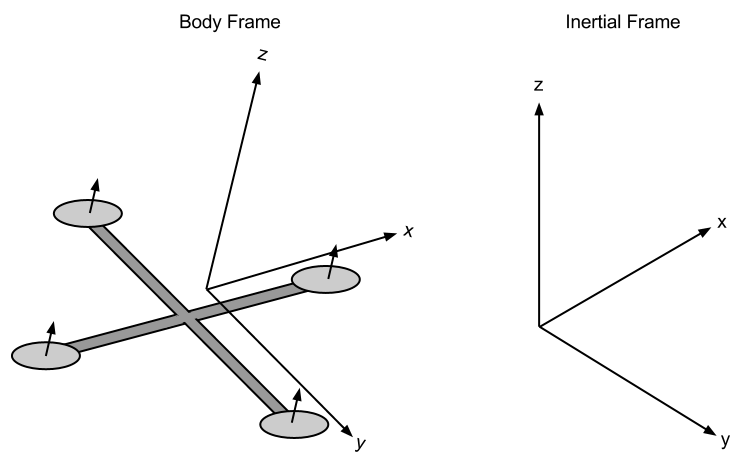
\includegraphics[width=0.6\textwidth]{images/Quadcopter_Coordinates.png}
	\caption{เฟรมอ้างอิงของโดรน}
	\label{fig:quadroter_coordinates}
\end{figure}

การควบคุมตำแหน่งและท่าทางของโดรนนั้น เราสามารถควบคุมได้โดยการสั่งให้มอเตอร์ทั้งสี่ตัวมีความเร็วที่แตกต่างกัน
เมื่อมอเตอร์หมุนด้วยความเร็วไม่เท่ากันจะทำให้เกิดแรงและโมเมนต์ขึ้นที่ตัวโดรน แรงยกนั้นจะเกิดขึ้นจากการหมุนมอเตอร์ทั้งหมด
ส่วนการเอียง Pitch (หมุนรอบแกน Y ของ Body frame), Roll (หมุนรอบแกน X ของ Body frame)
จะเกิดจากความแตกต่างระหว่างแรงยกของมอเตอร์ทั้งสี่ตัว แรงโน้มถ่วงของโลก และ Yaw (หมุนรอบแกน Z ของ Body frame)
เกิดจากการที่มอเตอร์หมุนด้วยความเร็วที่ไม่สมดุลกัน โดรนจะไม่หมุน Yaw หากมีมอเตอร์หมุนไปในทิศทางตรงกันข้ามกัน
ดังนั้นทำให้เราสามารถแบ่งใบพัดของโดรนออกเป็น 2 กลุ่ม แต่ละกลุ่มจะมีทิศทางการหมุนตรงข้ามกันและอยู่ฝั่งตรงกันข้ามกัน

\begin{itemize}
	\setlength\itemsep{-0.3em}
	\item ใบพัด หน้า และ หลัง (เลข 2 และเลข 4 ในรูปที่ \ref{fig:quadroter_rotordirection} ) จะหมุนทวนเข็มนาฬิกา CCW
	\item ใบพัด ซ้าย และ ขวา (เลข 1 และเลข 3 ในรูปที่ \ref{fig:quadroter_rotordirection} ) จะหมุนตามเข็มนาฬิกา CW
\end{itemize}

\begin{figure}[ht]
	\centering
	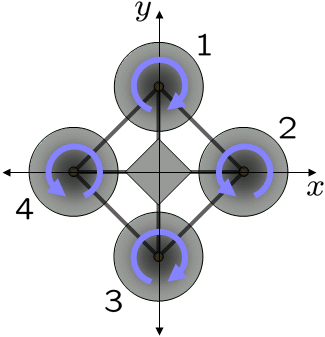
\includegraphics[width=0.4\textwidth]{images/Quadcopter_RotorDirection.png}
	\caption{ทิศทางการหมุนของแต่ละใบพัด}
	\label{fig:quadroter_rotordirection}
\end{figure}

การเคลื่อนที่ในปริภูมิของโดรนนั้นเราสามารถแบ่งได้ออกเป็น 2 ส่วนคือ การเคลื่อนที่ตามแนวแกน
และการเคลื่อนที่หมุนรอบแกน ในการอธิบายการเคลื่อนที่ของโดรนนั้น หากนับองศาอิสระจะได้ทั้งหมดเป็น 6 องศาอิสระ
โดย 6 องศาอิสระนี้คือ การเคลื่อนที่ตามแนวแกน 3 แกน (X Y Z) และการเคลื่อนที่หมุนรอบแกน (Roll Pitch Yaw)
การควบคุมการเคลื่อนที่ใน 6 องศาอิสระนั้นสามารถทำได้โดยปรับความเร็วการหมุนของมอเตอร์ให้มีความแตกต่างกัน
การเคลื่อนที่ไปข้างหน้า ถอยหลัง ไปด้านข้าง ขึ้นลง หมุนรอบ Roll Pitch Yaw,
ที่โดรนสามารถหมุนรอบแกน Yaw ได้นั้นเกิดจากทอร์คของมอเตอร์ทั้งสี่ ผลรวมของทอร์คจะส่งผลต่อความเร็วในการหมุนรอบแกน Yaw
หากมอเตอร์ทุกตัวหมุนด้วยความเร็วเท่ากัน ผลรวมทอร์คจะมีค่าเท่ากับศูนย์ทำให้โดรนไม่หมุน แต่ถ้ามอเตอร์หมุนด้วยความเร็วไม่เท่ากัน
จะทำให้ผลรวมทอร์คมีค่าไม่เท่ากับศูนย์จะส่งผลให้โดรนเกิดการหมุนรอบแกน Yaw ได้
ถ้ามอเตอร์ทุกตัวหมุนด้วยความเร็วเพิ่มขึ้นหรือลดลงพร้อมกันจะทำให้โดรนเคลื่อนที่ขึ้นหรือลงตามแนวดิ่ง
และด้วยการที่เรามี 4 Inputs แต่มี 6 Outputs นั้นทำให้การควบคุมโดรนเป็นแบบ Underactuated ซึ่งมีความซับซ้อนพอสมควร
เพื่อที่จะคอนโทรลโดรนได้นั้น ให้สมมุติว่าตัวโดรนเป็นวัตถุชิ้นเดียว (Rigid body) โครงสร้างมีความสมมาตร (Symmetric)
ความเร็วของแต่ละมอเตอร์ จะทำให้ใบพัดมีแรงยก เราสามารถบอกลักษณะการเคลื่อนที่ของโดรนได้ ดังรูปที่ \ref{fig:quadroter_movement}

\begin{figure}[!ht]
	\centering
	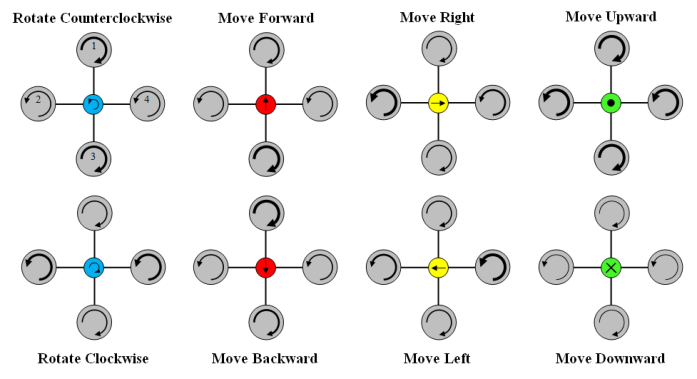
\includegraphics[width=0.95\textwidth]{images/Quadcopter_Movement.png}
	\caption{ทิศทางการเคลื่อนที่ของโดรนเมื่อมอเตอร์หมุนด้วยความเร็วต่างๆ}
	\label{fig:quadroter_movement}
\end{figure}

\clearpage
\subsection{Euler angles and Quaternions}
\subsection*{Euler angles}
มุมออยเลอร์เป็นมุม 3 มุมที่คิดโดย Leonhard Euler เพื่อที่จะเอาไว้ใช้อธิบายการเอียงของวัตถุในปริภูมิ
ใช้ตัวแปรเพียงแค่ 3 ตัวเท่านั้น การบอกมุมออยเลอร์สามารถบอกได้หลายวิธี ในที่นี้เราใช้ ZYX Euler angles
ในการอธิบายมุมเอียงของเฟรมอ้างอิงที่เราสนใจเทียบกับเฟรมอ้างอิงเฟรมอื่น มุมออยเลอร์เกิดจากการหมุนเฟรมรอบแกนสามแกน
มาหมุนเรียงต่อกัน ต่อไปจะเป็นการรวมแมทริกการหมุนสามแกนเข้าด้วยกัน

\begin{equation}
	{R_{x}(\phi) = \begin{bmatrix}
		1 & 0 & 0 \\
		0 & c(\phi) & -s(\phi) \\
		0 & s(\phi) & c(\phi)
		\end{bmatrix}}
	\label{equ:rotation_matrix_x}
\end{equation}

\begin{equation}
	{R_{y}(\theta) = \begin{bmatrix}
		c(\theta) & 0 & s(\theta) \\
		0 & 1 & 0 \\
		-s(\theta) & 0 & c(\theta)
		\end{bmatrix}}
	\label{equ:rotation_matrix_y}
\end{equation}

\begin{equation}
	{R_{z}(\psi) = \begin{bmatrix}
		c(\psi) & -s(\psi) & 0 \\
		s(\psi) & c(\psi) & 0 \\
		0 & 0 & 1 \\
		\end{bmatrix}}
	\label{equ:rotation_matrix_z}
\end{equation}

โดยที่ $c(\phi) = cos(\phi)$, $s(\phi) = sin(\phi)$, $c(\theta) = cos(\theta)$, $s(\theta) = sin(\theta)$, $c(\psi) = cos(\psi)$, $s(\psi) = sin(\psi)$
จากแมทริกการหมุนแสดงให้เห็นว่า \quotes{Inertial frame} และ \quotes{ฺBody frame}
มีความสัมพันธ์กันเป็นแมทริกการหมุนคือ $R_{zyx}(\phi,\theta,\psi)$
\begin{equation}
	\begin{array}{c}
		{R_{zyx}(\phi,\theta,\psi) = R_{z}(\psi)R_{y}(\theta)R_{x}(\phi)}\\
		{= \begin{bmatrix}
		c(\theta)c(\psi) & s(\phi)s(\theta)c(\psi)-c(\phi)s(\psi) & c(\phi)s(\theta)c(\psi)+s(\phi)s(\psi) \\
		c(\theta)s(\psi) & s(\phi)s(\theta)c(\psi)+c(\phi)s(\psi) & c(\phi)s(\theta)c(\psi)-s(\phi)c(\psi) \\
		-s(\theta)       & s(\phi)c(\theta)                       & c(\phi)c(\theta)                       \\
		\end{bmatrix}}
		\label{equ:rotation_matrix_zyx}
	\end{array}
\end{equation}

% แมทริกจากสมการที่ \ref{equ:rotation_matrix_zyx} เป็นแมทริกที่อธิบายถึงการหมุนจาก \quotes{ฺBody frame} ไปยัง \quotes{Inertial frame}
% ดังรูปที่ \ref{fig:quadroter_eulerangles}
% \begin{figure}[htbp]
% 	\centering
% 	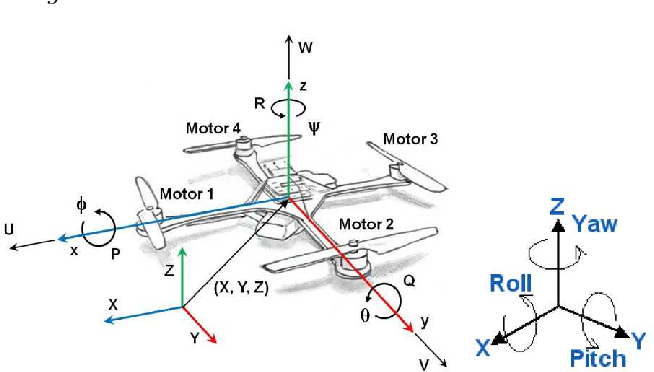
\includegraphics[width=0.65\textwidth]{images/Quadcopter_EulerAngles.png}
% 	\caption{ภาพแสดงการบอกแมทริกการหมุนของ Body frame}
% 	\label{fig:quadroter_eulerangles}
% \end{figure}

% \clearpage
\subsection*{Quaternions}
ในบางครั้งหรือบางกรณี Euler angles อาจจะทำให้เกิด Gimbal lock ได้
ซึ่งจะทำให้การควบคุมเสียไป 1 องศาอิสระ เพื่อที่จะหลีกเลี่ยงเหตุการณ์นี้จึงได้นำ quaternions มาใช้
quaternions ใช้เพื่อที่จะบอกมุมเอียงของวัตถุใดๆ ได้เหมือนกับ Euler angles
โดยที่เราสามารถแปลง Euler angles ให้เป็น quaternions ได้จากสมการที่ \ref{equ:euler2quat}

\begin{equation}
    {\begin{bmatrix} 
    q_1 \\ q_2 \\ q_3 \\ q_4
    \end{bmatrix} = \begin{bmatrix}
        c(\frac{\phi}{2})c(\frac{\theta}{2})c(\frac{\psi}{2})
        + s(\frac{\phi}{2})s(\frac{\theta}{2})s(\frac{\psi}{2}) \\[10pt]
        s(\frac{\phi}{2})c(\frac{\theta}{2})c(\frac{\psi}{2})
        + c(\frac{\phi}{2})s(\frac{\theta}{2})s(\frac{\psi}{2}) \\[10pt]
        c(\frac{\phi}{2})s(\frac{\theta}{2})c(\frac{\psi}{2})
        + s(\frac{\phi}{2})c(\frac{\theta}{2})s(\frac{\psi}{2}) \\[10pt]
        c(\frac{\phi}{2})c(\frac{\theta}{2})s(\frac{\psi}{2})
        + s(\frac{\phi}{2})s(\frac{\theta}{2})c(\frac{\psi}{2}) \\
		\end{bmatrix}}
	\label{equ:euler2quat}
\end{equation}

และเราสามารถที่จะเขียนแมทริกการหมุนให้อยู่ในรูปของ quaternions ได้ดังสมการที่ \ref{equ:quat2rot}
\begin{equation}
    {R_{zyx}(\phi,\theta,\psi) = \begin{bmatrix}
        q_1^2+q_2^2-q_3^2-q_4^2 & 2(q_2q_3-q_1q_4) & 2(q_1q_3+q_2q_4) \\[10pt]
        2(q_2q_3+q_1q_4) & q_1^2-q_2^2+q_3^2-q_4^2 & 2(q_3q_4-q_1q_2) \\[10pt]
        2(q_2q_4-q_1q_3) & 2(q_1q_2-q_3q_4) & q_1^2-q_2^2-q_3^2+q_4^2  \\
       \end{bmatrix}}
	\label{equ:quat2rot}
\end{equation}

\clearpage
\subsection{Qaudroter mathematical model}
ในส่วนนี้จะเป็นการอธิบายสมการการเคลื่อนที่ของโดรน โดยใช้สมการของ Newton และ Euler มาช่วยในการอธิบายพลวัต (Dynamics) ของโดรน
เพื่อใช้ทำแบบจำลอง (Simulating) และควบคุม (Controlling) ท่าทางของโดรนด้วย
เริ่มจากให้ $[\begin{matrix}x & y & z & \phi & \theta & \psi \end{matrix}]^T$ เป็นเวกเตอร์ที่บอกตำแหน่งและมุม (linear/angular position)
ของโดรนโดยเทียบจากเฟรมโลก (Inertial frame) และ $[\begin{matrix}u & v & w & p & q & r\end{matrix}]^T$ เป็นเวกเตอร์ที่บอกความเร็วเชิงเส้นและความเร็วเชิงมุม
(linear/angular velocity) ของโดนโดยเทียบจากเฟรมโดรน (Body frame) พลวัตของโดรนจะเปิดจากเฟรมอ้างอิงสองเฟรมนี้มีความสัมพันธ์กัน

\begin{equation}
	\begin{array}{c}
		{\nu = R\nu_{B}}               \\
		{\omega = T\omega_{B}}         
		\label{equ:equation_of_motion} 
	\end{array}
\end{equation}

โดยที่ $\nu = [\begin{matrix}\dot{x} & \dot{y} & \dot{z} \end{matrix}]^T$, $\omega = [\begin{matrix}\dot\phi & \dot\theta & \dot\psi \end{matrix}]^T$,
$\nu_{B} = [\begin{matrix}u & v & w \end{matrix}]^T$, $\omega_{B} = [\begin{matrix}p & q & r \end{matrix}]^T$ และ $T$
เป็นแมทริกการแปลงมุมการหมุน (angular transformation)
\begin{equation}
	{T = \begin{bmatrix}
		1 & s(\phi)t(\theta) & c(\phi)t(\theta) \\
		0 & c(\phi) & -s(\phi) \\
		0 & \dfrac{s(\phi)}{c(\theta)}  & \dfrac{c(\phi)}{c(\theta)} \\
		\end{bmatrix}}
	\label{equ:angular_transformation}
\end{equation}

โดยที่ $t(\theta) = tan(\theta)$ ดังนั้นเราจะได้สมการจลศาสตร์ (Kinematic model) ของโดรนเป็น
\begin{equation}
	{\begin{bmatrix}
		\dot{x}  \\
		\dot{y}  \\
		\dot{z} \\
		\dot{\phi} \\
		\dot{\theta} \\
		\dot{\psi} \\
		\end{bmatrix} = 
		\begin{bmatrix}
			w[s(\phi)s(\psi)+c(\phi)c(\psi)s(\theta)]-v[c(\phi)s(\psi)-c(\psi)s(\phi)s(\theta)]+u[c(\psi)c(\theta)] \\
			v[c(\phi)c(\psi)+s(\phi)s(\psi)s(\theta)]-w[c(\psi)s(\phi)-c(\phi)s(\psi)s(\theta)]+u[c(\theta)s(\psi)] \\
			w[c(\phi)c(\theta)]-u[s(\theta)]+v[c(\theta)s(\phi)]                                                    \\
			p+r[c(\phi)t(\theta)]+q[s(\phi)t(\theta)]                                                               \\
			q[c(\phi)]-r[s(\phi)]                                                                                   \\
			r\dfrac{c(\phi)}{c(\theta)}+q\dfrac{s(\phi)}{c(\theta)}                                                 \\
		\end{bmatrix}	}
	\label{equ:kinematic model}
\end{equation}

จากกฎของนิวตันระบุความสัมพันธ์ของแรงรวมที่กระทำต่อโดรนดังเมทริกซ์ต่อไปนี้

\begin{equation}
	{ m(\omega_B\wedge \nu_B+\dot{\nu_B})=\mathbf{f}_B}
	\label{equ:total force}
\end{equation}

โดย $m$ คือน้ำหนักของโดรน , $\wedge$ คือ cross product และ $\mathbf{f}_B=\begin{bmatrix}f_x & f_y & f_z \end{bmatrix}^T \in \mathbf{R}^3$ 
คือแรงรวม
\\ จากสมการออยเลอร์ ให้แรงบิดรวมที่ใช้กับโดรน เป็นไปดังนี้

\begin{equation}
	{
		I.\dot{\omega}_B+\omega_B\wedge(I.\omega_B)=\mathbf{m}_B
	}
	\label{equ:total force}
\end{equation}
\\
โดย $\mathbf{m}_B=\begin{bmatrix}m_x & m_y & m_z\end{bmatrix}^T \in \mathbf{R}^3$ เป็นแรงบิดรวม และ $I$ เป็นเมทริกซ์ของความเฉื่อย :
\begin{equation}
	{
		I = \begin{bmatrix}I_x & 0 & 0 \\
		0   & I_y & 0 \\
		0   & 0 & I_z \\
		\end{bmatrix} \wedge \mathbf{R}^{3\times3}
	}
	\label{equ:inertia matrix}
\end{equation}

ดังนั้น จะได้ dynamic model ของโดรนโดยอ้างอิง body frame ดังนี้
\begin{equation}
	{
		\begin{bmatrix}	f_x \\
			f_y \\
			f_z \\
			m_x \\
			m_y \\
			m_z \\   
		\end{bmatrix} = 
		\begin{bmatrix}	m(\dot{u}+qw-rv) \\
			m(\dot{v}-pw+ru)       \\
			m(\dot{w}+pv-qu)       \\
			\dot{p}I_x-qrI_y+qrI_z \\
			\dot{q}I_y+prI_x-prI_z \\
			\dot{r}I_z-pqI_x+pqI_y \\   
		\end{bmatrix}
	}
	\label{equ:dynamic model}
\end{equation}

% ซึ่งระบบต่าง ๆ จะเป็นไปตามสมการข้างต้นเมื่อกำหนดให้จุด origin และ body frame ตรงกับจุดเซนทรอยด์และ principal axes ของโดรน

\clearpage
\subsection{Motor model}
ในแต่ละใบพัดของ quadrotor จะให้แรงที่มีทิศทางตรงข้ามกับแกน $Z$ ของ body frame
แรงที่เกิดจากการหมุนจะทำให้เกิดแรงบิดรอบแนวแกน roll pitch yaw โดยแรงและแรงบิดจะขึ้นอยู่กับความเร็วของใบพัดและค่าคงที่ค่าหนึ่ง
ซึ่งสามารถแสดงความสัมพันธ์ของแรงได้ดังสมการที่ \ref{equ:force_equ} และความสัมพันธ์ของแรงบิดได้ดังสมการที่ \ref{equ:torque_equ}

\begin{equation}
    {F_i = k_f\Omega_i^2}
	\label{equ:force_equ}
\end{equation}

\begin{equation}
    {T_i = -k_tsgn(i)\Omega_i^2}
	\label{equ:torque_equ}
\end{equation}

โดยที่ตัวห้อย $i$ จะแสดงถึงลำดับของใบพัดแต่ละตัว $\Omega_i$ แสดงถึงความเร็วการหมุนของใบพัด $i$
$k_f$ และ $k_t$ เป็นค่าคงที่การคูณของแรงและแรงบิด $sgn$ เป็นฟังก์ชันที่ใช้บอกทิศทางการหมุนของใบพัดที่มีความแตกต่างกันตามการติดตั้ง
แรงทั้งหมดที่เกิดบน quadrotor สามารถที่จะเขียนสมการให้อยู่ในรูปของความเร็วการหมุนของใบพัดคูณกับแมทริกการแปลง $M$ ดังสมการที่ \ref{equ:map_force_torque}

\begin{equation}
    {\begin{bmatrix} 
    F \\[10pt] \tau_\phi \\[10pt] \tau_\theta \\[10pt] \tau_\psi \\
    \end{bmatrix} = M\begin{bmatrix}
    \Omega_1^2 \\[10pt]
    \Omega_2^2 \\[10pt]
    \Omega_3^2 \\[10pt]
    \Omega_4^2 \\       
    \end{bmatrix}}
	\label{equ:map_force_torque}
\end{equation}

โดยที่ แมทริกการแปลง $M$ มีการกำหนดไว้ดังสมการที่ \ref{equ:map_matrix}

\begin{equation}
    {M = \begin{bmatrix}
    k_f & k_f & k_f & k_f \\[10pt]
    \frac{k_fd}{\sqrt{2}} & -\frac{k_fd}{\sqrt{2}} & -\frac{k_fd}{\sqrt{2}} & \frac{k_fd}{\sqrt{2}}  \\[10pt]
    \frac{k_fd}{\sqrt{2}} & \frac{k_fd}{\sqrt{2}} & -\frac{k_fd}{\sqrt{2}} & -\frac{k_fd}{\sqrt{2}}  \\[10pt]
    k_t & -k_t & k_t & -k_t \\
    \end{bmatrix}}
	\label{equ:map_matrix}
\end{equation}

โดยที่ $\Omega_i^2$ เป็นความเร็วการหมุนของใบพัดกำลังสอง และ $d$ คือระยะทางจากจุดศูนย์กลางมวลของ quadrotor ไปถึงจุดกึ่งกลางของใบพัด





% https://www2.eecs.berkeley.edu/Pubs/TechRpts/2012/EECS-2012-241.pdf
% https://www.kth.se/polopoly_fs/1.588039!/Thesis%20KTH%20-%20Francesco%20Sabatino.pdf

\clearpage
\section{Linear Quadratic Regulator}
ในส่วนนี้จะกล่าวถึงตัวควบคุม LQR ซึ่งเป็นส่วนที่ใช้ในการควบคุม quadrotor โดยจะแบ่งออกเป็นสองส่วนควบคุม
ตำแหน่งและทิศทางการหมุนสามารถอ้างอิงและควบคุมได้โดยตรง ส่วน Roll และ Pitch ไม่สามารถควบคุมได้โดยตรง
แต่จะควบคุมผ่านตำแหน่ง x และ y

ตัวควบคุม LQR ถูกพัฒนามาเพื่อใช้กับระบบที่มีการควบคุม inputs และ output เพื่อที่จะหาตัวควบคุม state feedback
ที่มีประสิทธิ์ภาพมากที่สุด

สมมุติให้ Linear state spcae model ของ quadrotor เป็นดังสมการที่ \ref{equ:linear_state_spcae_model}

\begin{equation}
    {\dot{x} = Ax + Bu}
	\label{equ:linear_state_spcae_model}
\end{equation}

โดยที่ $A$ เป็น state matrix, $B$ เป็น input matrix, $x$ เป็น state vector ที่มีจำนวนตัวเท่ากับ $n$ ตัว,
และ $u$ เป็น input vector ที่มีจำนวนตัวเท่ากับ $m$ ตัว โดยทั้ง $A$, $B$ จะต้องตรวจสอบก่อนว่าระบบเราสามารถที่จะควบคุมได้หรือไม่

ตัวควบคุม LQR สามารถออกแบบให้มีประสิทธิ์ภาพสูงสุดได้โดยที่ยังควบคุมระบบได้ เป้าหมายหลักก็คือการหาค่า feedback gain $K$,
ผลลัพธ์การควบคุมที่ดีที่สุดโดยการ minimizes cost function ตามสมการที่ \ref{equ:cost_func}
\begin{equation}
    {๋J = \int_{0}^{\infty} (x^TQx+u^TRu) dt}
	\label{equ:cost_func}
\end{equation}

โดยที่ $Q$ และ $R$ เป็นนำหนักของ input และ state ถ้าหาก $Q$ มีค่ามากหมายความว่าความถูกต้องของ state มีความสำคัญมาก
และควรจะมีค่าความผิดพลาดน้อยเพื่อที่จะทำให้ cost ของ J น้อย และ $R$ ก็คล้ายๆกันหากมีค่ามากหมายความว่าการใช้ input มีความสำคัญมาก

ผลลัพธ์ของ control input จาก feedback gain ดังสมการที่ \ref{equ:feedback_gain}
\begin{equation}
    {๋u = -Kx}
	\label{equ:feedback_gain}
\end{equation}

โดยที่ $K$ เป็น feedback gain และสามารถหาได้จากสมการที่ \ref{equ:feedback_gain_equ}
\begin{equation}
    {๋K = R^{-1}B^TP}
	\label{equ:feedback_gain_equ}
\end{equation}

โดยที่ $P$ เป็นสิ่งที่เราต้องหาเพื่อใช้ในการหา $K$ จากการแก้สมการของ Riccati ดังสมการที่ \ref{equ:riccati_algebraic}
\begin{equation}
    {๋A^TP+PA+Q-PBR^{-1}B^TP = 0}
	\label{equ:riccati_algebraic}
\end{equation}



\clearpage
\section{Hector Quadrotor ROS Stack}
Hector Quadrotor เป็น ROS stacks (stack เป็นการรวบรวม packages ที่มีหลากหลายฟังก์ชันเอาไว้ด้วยกัน)
โดยภายในประกอบไปด้วย ROS packages ดังต่อไปนี้
\begin{enumerate}[label=\arabic*), leftmargin=1.5cm]
	\setlength\itemsep{-0.25em}
	\item hector\_quadrotor\_description
	\item hector\_quadrotor\_gazebo
	\item hector\_quadrotor\_teleop
	\item hector\_quadrotor\_gazebo\_plugin
\end{enumerate}


% \paragraph*{}
% เป็นแพกเกจที่มีไฟล์ quadrotor URDF model หลากหลายประเภท
% \paragraph*{hector\_quadrotor\_gazebo}
% เป็นแพกเกจที่มีไฟล์ launch สำหรับการทำ simulation ด้วยโปรแกรม Gazebo
% \paragraph*{hector\_quadrotor\_teleop}
% เป็นแพกเกจที่มีไฟล์ node สำหรับควบคุม quadrotor ด้วย gamepad
% \paragraph*{title}

\subsection{hector\_quadrotor\_description}
package นี้ให้ URDF model ของ quadrotor มี visual geometry เป็นไฟล์ COLLADA และ collision geometry เป็นไฟล์ STL
โดยจะเป็นส่วนเสริมที่ทำให้เราสามารถที่จะใช้ model ในโปรแกรม Gazebo ได้\footnote{http://wiki.ros.org/hector\_quadrotor\_description}

% \vspace{20pt}
\paragraph*{quadroter\_base.urdf.xacro}
เป็นไฟล์ xacro ของโมเดลขั้นพื้นฐานของ quadroter
\paragraph*{quadrotor.urdf.xacro}
เป็นไฟล์ xacro สำหรับการแสดงโมเดลขั้นพื้นฐานโดยไม่มีเซนเซอร์เพิ่มเติม
\paragraph{quadrotor\_hokuyo\_utm30lx.urdf.xacro}
เป็นไฟล์ xacro สำหรับการแสดงโมเดลขั้นพื้นฐานโดยเพิ่มเติมเซนเซอร์ Hokuyo เข้าไปสำหรับแสกนสิ่งแวดล้อม

\begin{figure}[!ht]
	\centering
	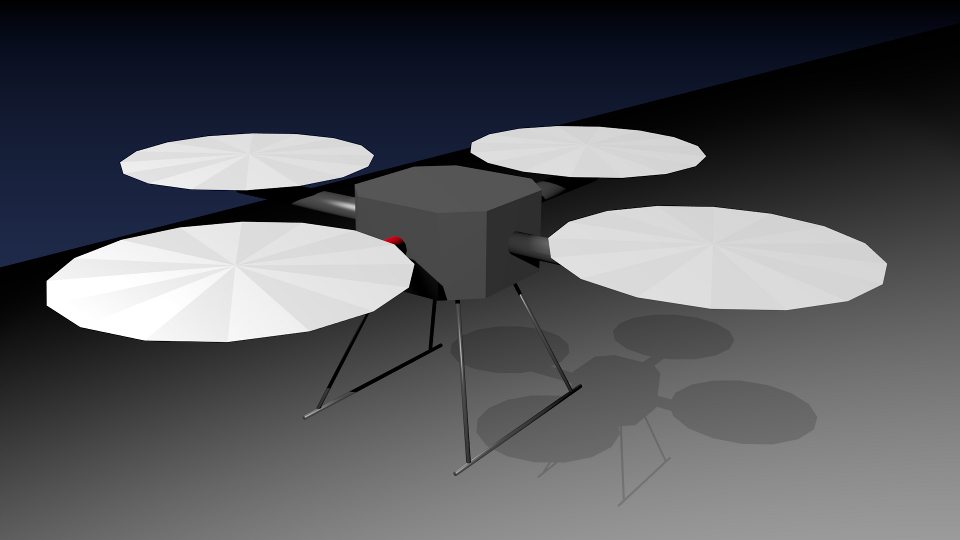
\includegraphics[width=0.85\textwidth]{images/hector_quadrotor_render.png}
	\caption{ภาพ quadrotor ที่ render ด้วย Blender}
	\label{fig:hector_quadrotor_render}
\end{figure}

\subsection{hector\_quadrotor\_gazebo}
package นี้ให้ quadroter model ที่มาจากไฟล์ urdf และมาแสดงผลในโปรแกรม Gazebo โดย features\footnote{http://wiki.ros.org/hector\_quadrotor\_gazebo} ที่มีคือ
\begin{enumerate}[label=\arabic*), leftmargin=1.5cm]
	\setlength\itemsep{-0.25em}
	\item Colored COLLADA quadrotor mesh model (.dae)
	\item URDF description
	\item Publishing of ground truth pose and simulated imu data
	\item Spawnable in Gazebo
	\item Controller สำหรับใช้ใน Gazebo โดยสามารถควบคุมผ่าน geometry\_msgs/Twist message ใน topic 'cmd\_vel'
\end{enumerate}

\clearpage
\subsection{hector\_quadrotor\_teleop}
package นี้จะทำให้เราสามารถที่จะควบคุม quadrotor ผ่าน gamepad ได้ โดยจะมี node ที่ publish geometry\_msgs/Twist message ไปที่ topic 'cmd\_vel'
ปัจจุบันมี gamepad 2 ชนิดที่นำมาใช้ได้ก็คือ
\begin{enumerate}[label=\arabic*), leftmargin=1.5cm]
	\setlength\itemsep{-0.25em}
	\item logitech\_gamepad.launch สำหรับ Logitech gamepads
	\item xbox\_controller.launch สำหรับ Xbox controller gamepads 
\end{enumerate}
แต่หากต้องการใช้งานนอกเหนือจากนี้ สามารถที่จะสร้าง node ขึ้นมาใหม่ได้

\vspace{20pt}
\subsection{hector\_quadrotor\_gazebo\_plugin}
package นี้เป็นส่วนเสริมของ Gazebo ที่จะทำให้มีเซนเซอร์ต่างๆเข้ามาในระบบได้
\paragraph*{Barometer Plugin}
เป็นส่วนเสริมที่จำลองเซนเซอร์ัที่ใช้วัดความสูงของ quadrotor โดยมีพื้นฐานมาจากการวัด barometric pressure
\paragraph*{Simple Controller Plugin}
package นี้เป็นส่วนเสริมของ Gazebo ที่จะทำให้เราสามารถควบคุม Velocities และ Yaw rate ได้โดยการคำนวณ แรงและแรงบิด
โดยในปัจจุบันยังไม่สามารถที่จะควบคุมตำแหน่ง ทิศทางการหันหัว และความสูงได้ แต่สามารถที่จะเขียนทับเข้าไปได้
\paragraph*{Quadrotor Propulsion Plugin / Quadrotor Aerodynamics Plugin}
package นี้เป็นส่วนเสริมของ Gazebo ที่จะทำให้เราสามารถควบคุมการหมุนของใบพัด quadroter ได้ โดยการควบคุม voltages ของมอเตอร์
และยังจำลอง wind vector ได้อีกด้วย
\paragraph*{Matlab Compilation}
ในการเขียนสมการต่างๆของระบบ quadroter มักจะนิยมใช้ Matlab script และคอมไพล์เป็น C libraries โดยใช้ Matlab Coder
ส่วนเสริมตัวนี้จะช่วยทำให้สามารถเชื่อมต่อกับ Matlab ได้

\begin{figure}[!ht]
	\centering
	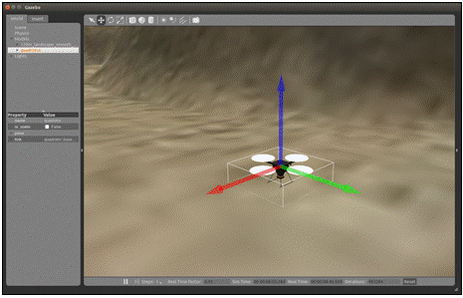
\includegraphics[width=0.85\textwidth]{images/hector_quadrotor_gazebo.png}
	\caption{ภาพ quadrotor ในโปรแกรม Gazebo}
	\label{fig:hector_quadrotor_gazebo}
\end{figure}


\chapter{Simulation}

\section{Quadrotor simulation model}
เราได้ใช้โปรแกรม Simulink จำลองการทำงานของ quadrotor โดยจะแบ่งออกเป็นสองส่วน คือ
\vspace{-10pt}
\begin{enumerate}[label=\arabic*), leftmargin=1.5cm]
	\setlength\itemsep{-0.25em}
	\item อัตราการเปลี่ยนแปลงความเร่งเชิงเส้นโดยถูกเขียนขึ้นจากทฤษฏีที่กล่าวไปในบทที่ 2
	\item อัตราการเปลี่ยนแปลงความเร่งเชิงมุมโดยถูกเขียนขึ้นจากทฤษฏีที่กล่าวไปในบทที่ 2
\end{enumerate}
\vspace{-15pt}
\begin{figure}[!ht]
	\centering
	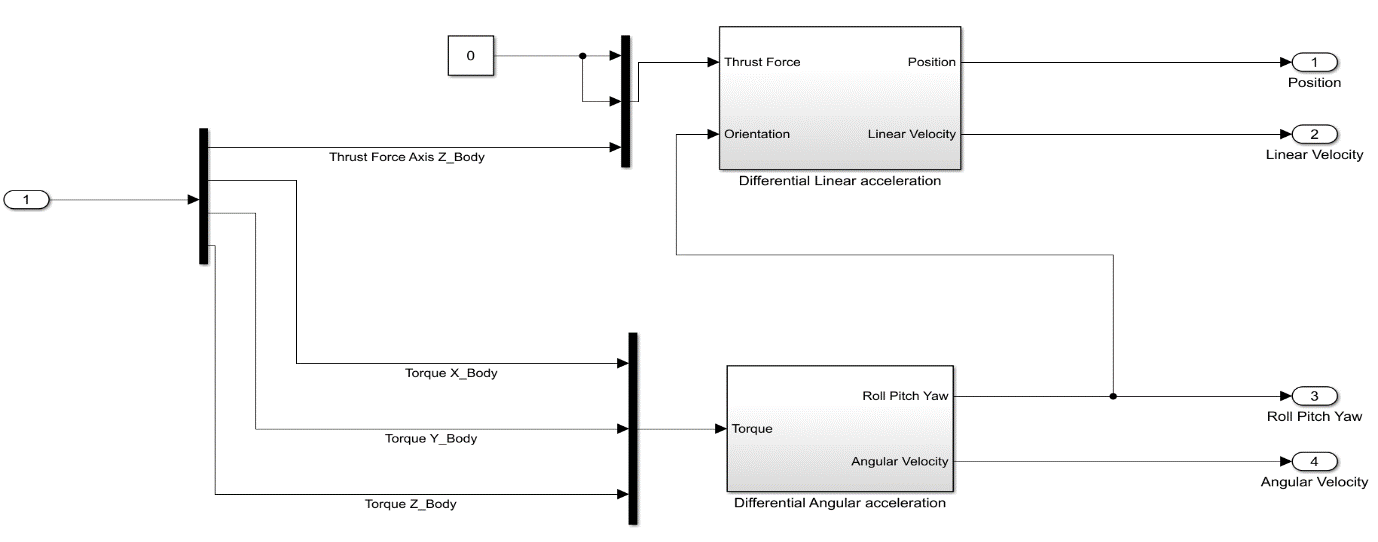
\includegraphics[width=0.8\textwidth]{images/simulink/sim_dynamic_all.png}
	\caption{แบบจำลอง quadrotor ในโปรแกรม simulink}
\end{figure}

\subsection{อัตราการเปลี่ยนแปลงความเร่งเชิงเส้น}
\begin{figure}[!ht]
	\centering
	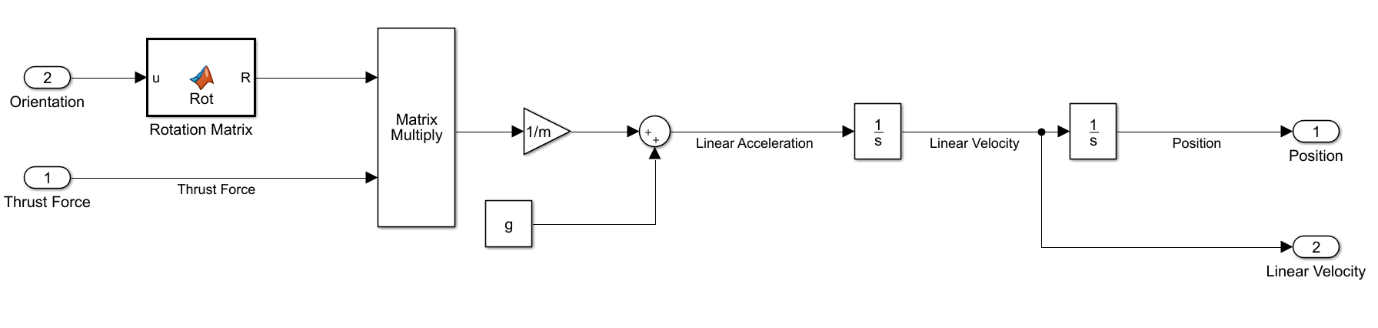
\includegraphics[width=0.95\textwidth]{images/simulink/linear_acce.png}
	\caption{อัตราการเปลี่ยนแปลงความเร่งเชิงเส้น}
\end{figure}
\vspace{-10pt}
\paragraph*{Input}
เป็นแรงขับที่กระทำกับ quadrotor และทิศทางการหมุนของ quadrotor
\paragraph*{Output}
เป็นตำแหน่งและความเร็วเชิงเส้นของ quadrotor
\vspace{15pt}
\subsection{อัตราการเปลี่ยนแปลงความเร่งเชิงมุม}
\begin{figure}[!ht]
	\centering
	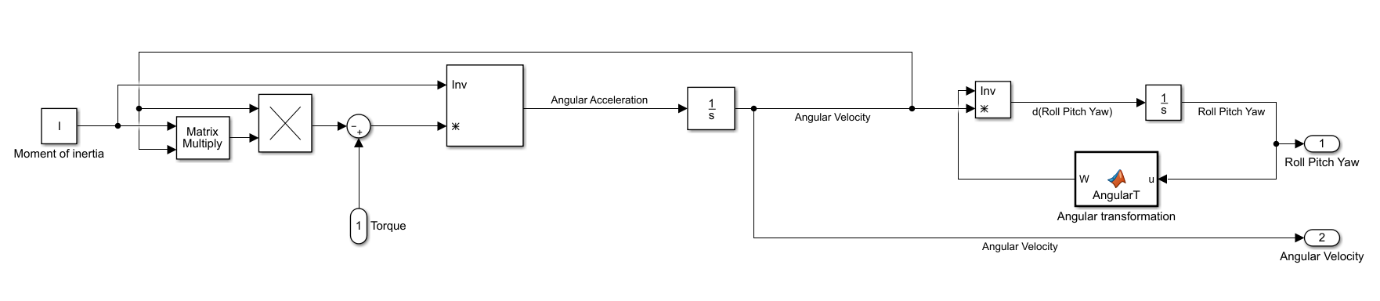
\includegraphics[width=0.95\textwidth]{images/simulink/angular_acce.png}
	\caption{อัตราการเปลี่ยนแปลงความเร่งเชิงมุม}
\end{figure}
\vspace{-10pt}
\paragraph*{Input}
เป็นแรงบิดที่กระทำกับ quadrotor
\paragraph*{Output}
เป็นทิศทางการหมุนของ quadrotor และความเร็วเชิงมุมของ quadrotor

\clearpage
\subsection{ผลการทดลอง}
กำหนดค่าเริ่มต้นต่างๆของ quadrotor ที่ใช้กับการทดลองดังนี้


\begin{center}
    \begin{tabular}{ | c | c | c | } 
    \hline
    ตัวแปร & ค่า & หน่วย \\ 
    \hline
    \hline
    $I_x$ & 0.01152 & $kgm^2$ \\ 
    \hline
    $I_y$ & 0.01152 & $kgm^2$ \\
    \hline
    $I_z$ & 0.0218 & $kgm^2$ \\
    \hline
    $g$ & 9.80665 & $m/s^2$ \\
    \hline
    $m$ & 1.477 & $kg$ \\
    \hline
    $L$ & 0.26 & $m$ \\
    \hline
    \end{tabular}
\end{center}

\subsubsection{Hover quadrotor}
ทดลอง Simulation โดยการใส่แรงขับที่กระทำให้ quadrotor สามารถลอยตัวอยู่ได้โดยไม่ร่วงลงตามแรงโน้มถ่วงของโลก

\begin{equation}
    \begin{array}{c}
    {F = ma}\\
    {F = 1.477 \times 9.80665}
    \label{equ:newton_law}
    \end{array}
\end{equation}
\begin{center}
    \begin{tabular}{ | c | c | c | } 
    \hline
    Thrust force Z & 14.48442205 & $Nm$ \\ 
    \hline
    Torque X & 0 & $Nm$ \\ 
    \hline
    Torque Y & 0 & $Nm$ \\ 
    \hline
    Torque Z & 0 & $Nm$ \\ 
    \hline
    \end{tabular}
\end{center}
\begin{figure}[!ht]
	\centering
	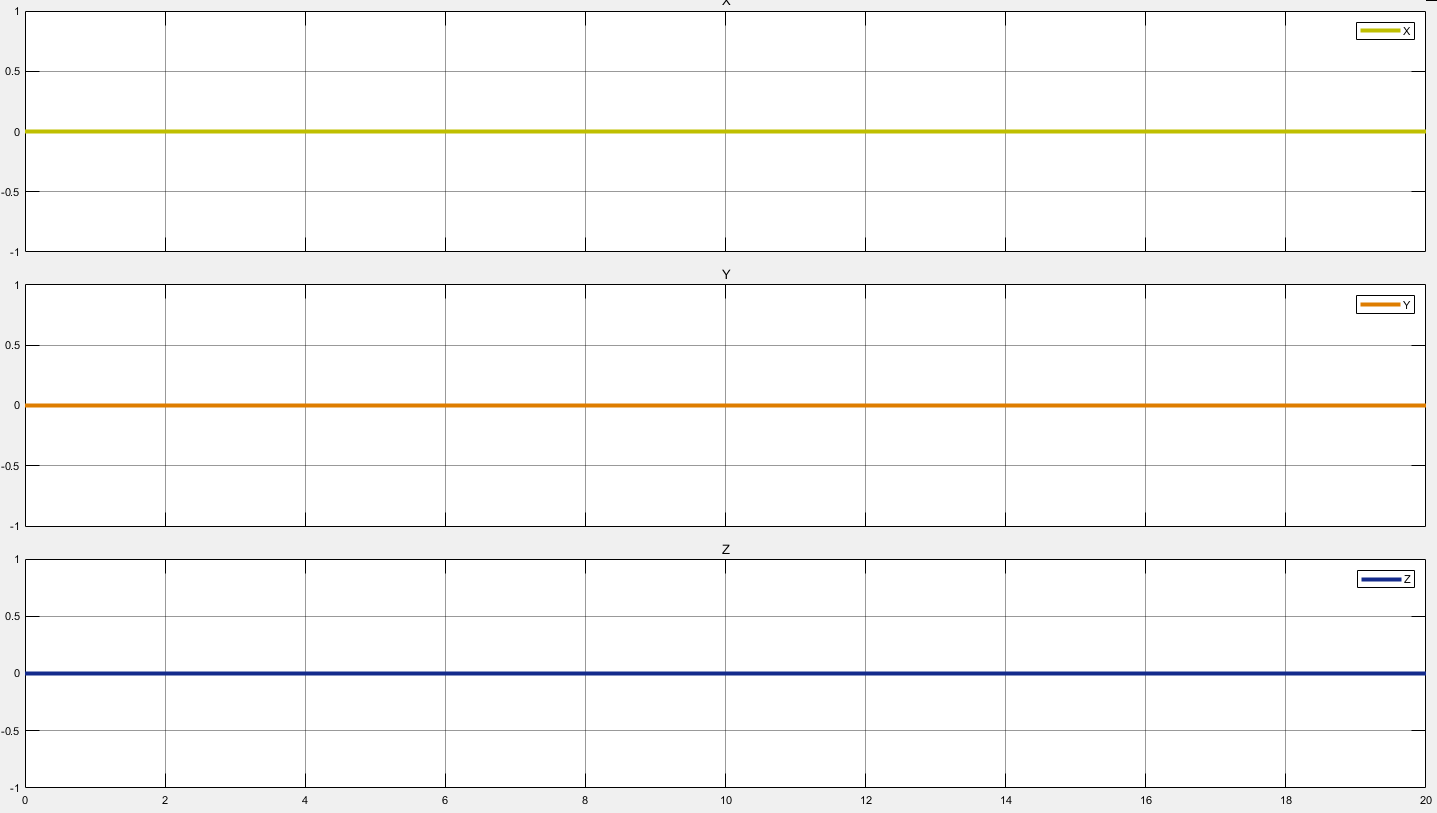
\includegraphics[width=0.95\textwidth]{images/simulink/test_hover.png}
	\caption{กราฟแสดงตำแหน่งของ quadrotor}
\end{figure}

จากผลการทดลอง quadrotor สามารถลอยอยู่ได้ที่ตำแหน่ง $x=0$, $y=0$ และ $z=0$ โดยไม่ร่วงลงมาตามแรงโน้มถ่วงของโลก

\clearpage
\subsubsection{Climb up quadrotor}
ทดลอง Simulation โดยการใส่แรงขับที่กระทำให้ quadrotor สามารถลอยตัวขึ้นไปในอากาศได้

\begin{equation}
    \begin{array}{c}
    {F > ma}\\
    {F > 1.477 \times 9.80665}
    \label{equ:newton_law}
    \end{array}
\end{equation}
\begin{center}
    \begin{tabular}{ | c | c | c | } 
    \hline
    Thrust force Z & 15.48442205 & $Nm$ \\ 
    \hline
    Torque X & 0 & $Nm$ \\ 
    \hline
    Torque Y & 0 & $Nm$ \\ 
    \hline
    Torque Z & 0 & $Nm$ \\ 
    \hline
    \end{tabular}
\end{center}
\begin{figure}[!ht]
	\centering
	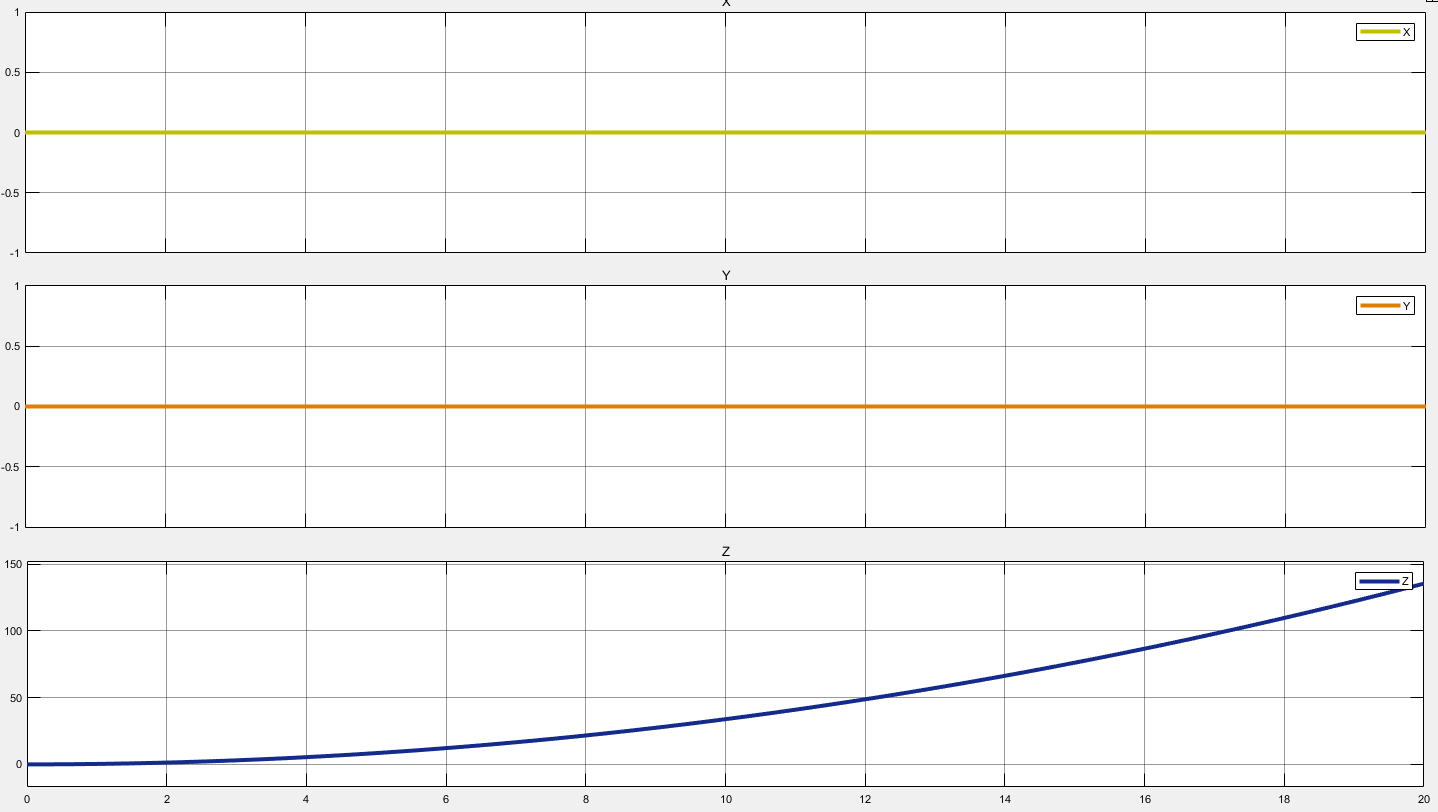
\includegraphics[width=0.95\textwidth]{images/simulink/test_climbup.png}
	\caption{กราฟแสดงตำแหน่งของ quadrotor}
\end{figure}

จากผลการทดลอง quadrotor สามารถเคลื่อนที่ลอยขึ้นไปในทิศทางตามแนวแกน Z ได้

\clearpage
\section{Simulation กับตัวควบคุม Linear Quadratic Regulator}
ในส่วนของการทดลองตัวควบคุมจะแบ่งออกเป็นสามส่วนคือ
\vspace{-10pt}
\begin{enumerate}[label=\arabic*), leftmargin=1.5cm]
	\setlength\itemsep{-0.25em}
    \item Altitude control
    \item Attitude control
    \item X Y Position control
\end{enumerate}
\vspace{-15pt}
\begin{figure}[!ht]
	\centering
	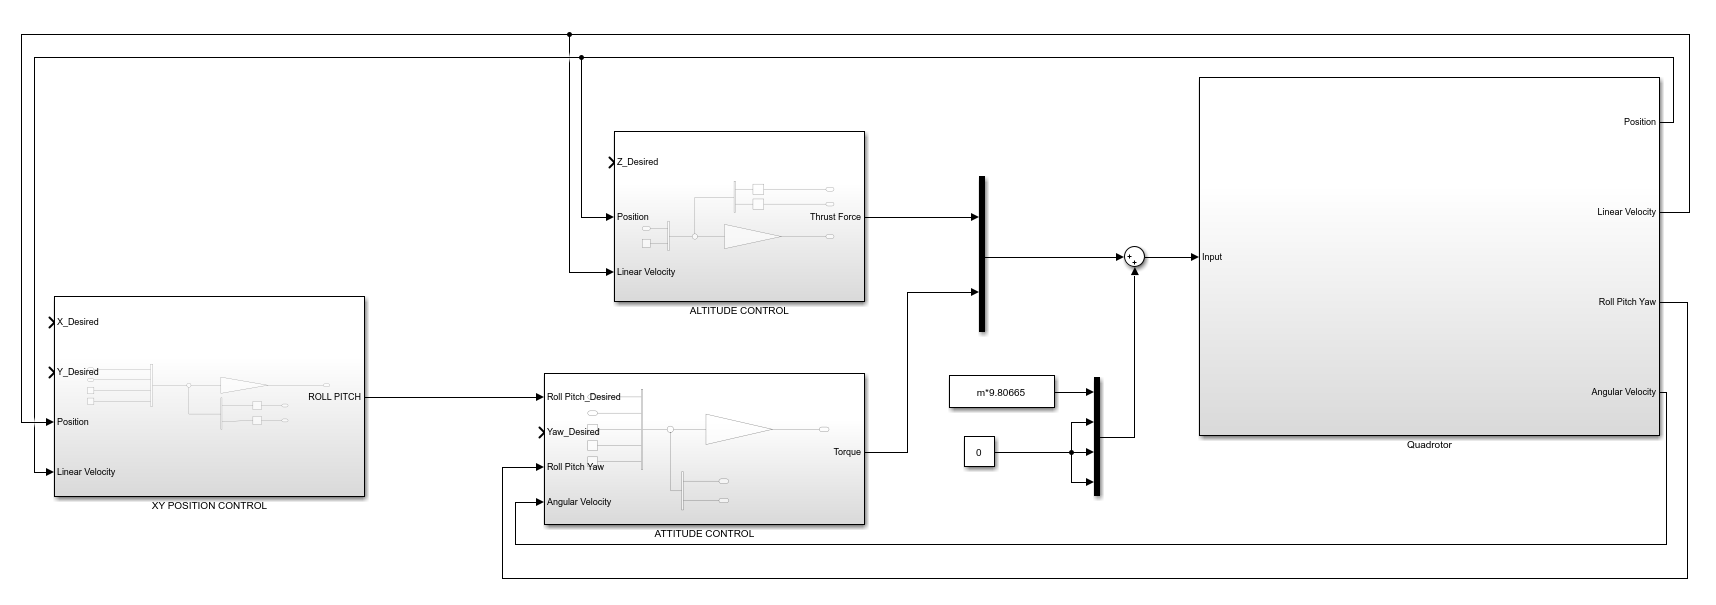
\includegraphics[width=0.8\textwidth]{images/simulink/lqr_all.png}
	\caption{แบบจำลองตัวควบคุม LQR ของ quadrotor ในโปรแกรม simulink}
\end{figure}

\subsection{Altitude control}
มี state และ input คือ
\begin{equation}
    {\vec{x}=\begin{bmatrix}
        z \\ v_z \\
    \end{bmatrix}, u = F_z}
\end{equation}

\paragraph*{การทดลองครั้งที่ 1}
กำหนดค่าน้ำหนักเมทริก $Q$ กับ $R$ ให้กับ Altitude control ดังนี้
\begin{equation}
    \begin{array}{c}
    {Q_{Altitude}=diag(\begin{bmatrix}
        1 & 1 \\
    \end{bmatrix})}\\[10pt]
    {R_{Altitude} = 1}\\[10pt]
    {K_{Altitude} = \begin{bmatrix}
        1 & 1.9885 \\
    \end{bmatrix}} \\
    \end{array}
\end{equation}

\begin{figure}[!ht]
	\centering
	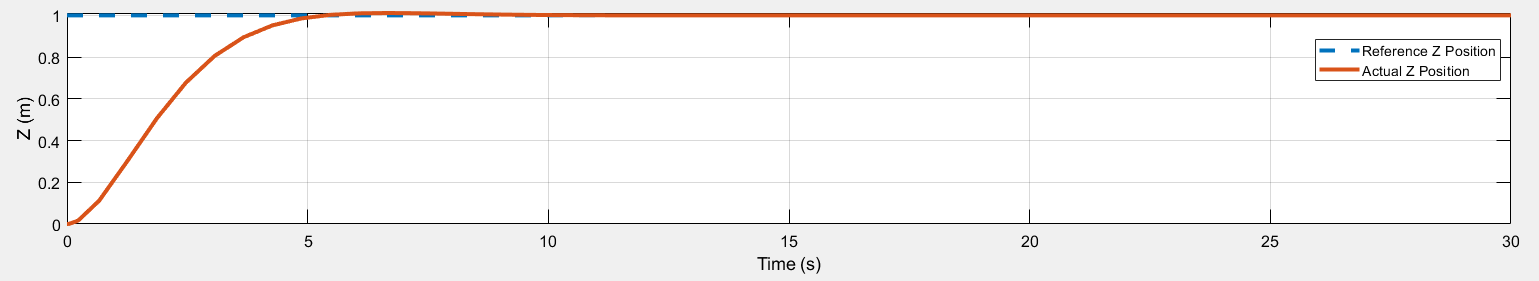
\includegraphics[width=0.8\textwidth]{images/simulink/altitude_control1.png}
	\caption{ผลการทดสอบ Altitude control ครั้งที่ 1}
\end{figure}

จากกราฟจะเห็นได้ว่าตำแหน่งตามแนวแกน Z ของ quadrotor สามารถลู่เข้าตำแหน่งที่ต้องการได้และใช้เวลาไปประมาณ 5 วินาที

\paragraph*{การทดลองครั้งที่ 2}
ต้องการให้ตำแหน่งตามแนวแกน Z ของ quadrotor ลู่เข้าสู่ตำแหน่งที่ต้องการได้เร็วขึ้น จึงได้กำหนดค่าน้ำหนักเมทริก
$Q$ กับ $R$ ขึ้นใหม่ดังนี้ 
\begin{equation}
    \begin{array}{c}
    {Q_{Altitude}=diag(\begin{bmatrix}
        10 & 1 \\
    \end{bmatrix})}\\[10pt]
    {R_{Altitude} = 1}\\[10pt]
    {K_{Altitude} = \begin{bmatrix}
        3.1623 & 3.2158 \\
    \end{bmatrix}} \\[10pt]
    \end{array}
\end{equation}

\begin{figure}[!ht]
	\centering
	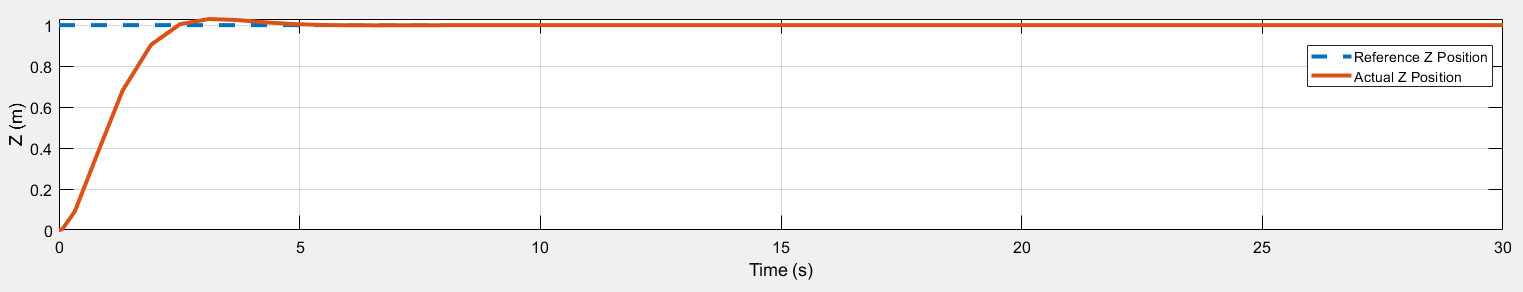
\includegraphics[width=0.8\textwidth]{images/simulink/altitude_control2.png}
	\caption{ผลการทดสอบ Altitude control ครั้งที่ 2}
\end{figure}
 
จากกราฟจะเห็นได้ว่าตำแหน่งตามแนวแกน Z ของ quadrotor สามารถลู่เข้า ณ ตำแหน่งที่ 1 เมตรเร็วขึ้น แต่มีการเกิด Overshoot ขึ้นเล็กน้อย

\subsection{Attitude control}
มี state และ input คือ
\begin{equation}
    {\vec{x}=\begin{bmatrix}
        \phi \\ \theta \\ \psi \\ p \\ q \\ r \\
    \end{bmatrix}, \vec{u} = \begin{bmatrix}
        \tau_x \\ \tau_y \\ \tau_z \\
    \end{bmatrix}}
\end{equation}

\paragraph*{การทดลองครั้งที่ 1}
กำหนดค่าน้ำหนักเมทริก $Q$ กับ $R$ ให้กับ Attitude control ดังนี้
\begin{equation}
    \begin{array}{c}
    {Q_{Altitude}=diag(\begin{bmatrix}
        1 & 1 & 1 & 1 & 1 & 1\\
    \end{bmatrix})}\\[10pt]
    {R_{Altitude} = diag(\begin{bmatrix}
        1 & 1 & 1\\
    \end{bmatrix})}\\[10pt]
    {K_{Altitude} = \begin{bmatrix}
        3.1623 & 3.2158 \\
    \end{bmatrix}} \\[10pt]
    \end{array}
\end{equation}
\clearpage
\section{Gazebo and Rviz}
ทดสอบการทำงานของโปรแกรม Matlab โดยจำลองในโปรแกรม Gazebo และแสดงผลภาพใน Rviz
การทดสอบแบ่งเป็น 3 ตัวอย่าง
\begin{enumerate}[label=\arabic*), leftmargin=1.5cm]
	\setlength\itemsep{-0.25em}
	\item สั่งให้ quadrotor บินขึ้นเหนือพื้น
	\item สั่งให้ quadrotor บินวนเป็นเกลียว
	\item สั่งให้ quadrotor บินเป็นรูปดาว
\end{enumerate}

\begin{figure}[!ht]
    \centering
    \begin{subfigure}[b]{0.8\textwidth}
        \centering
        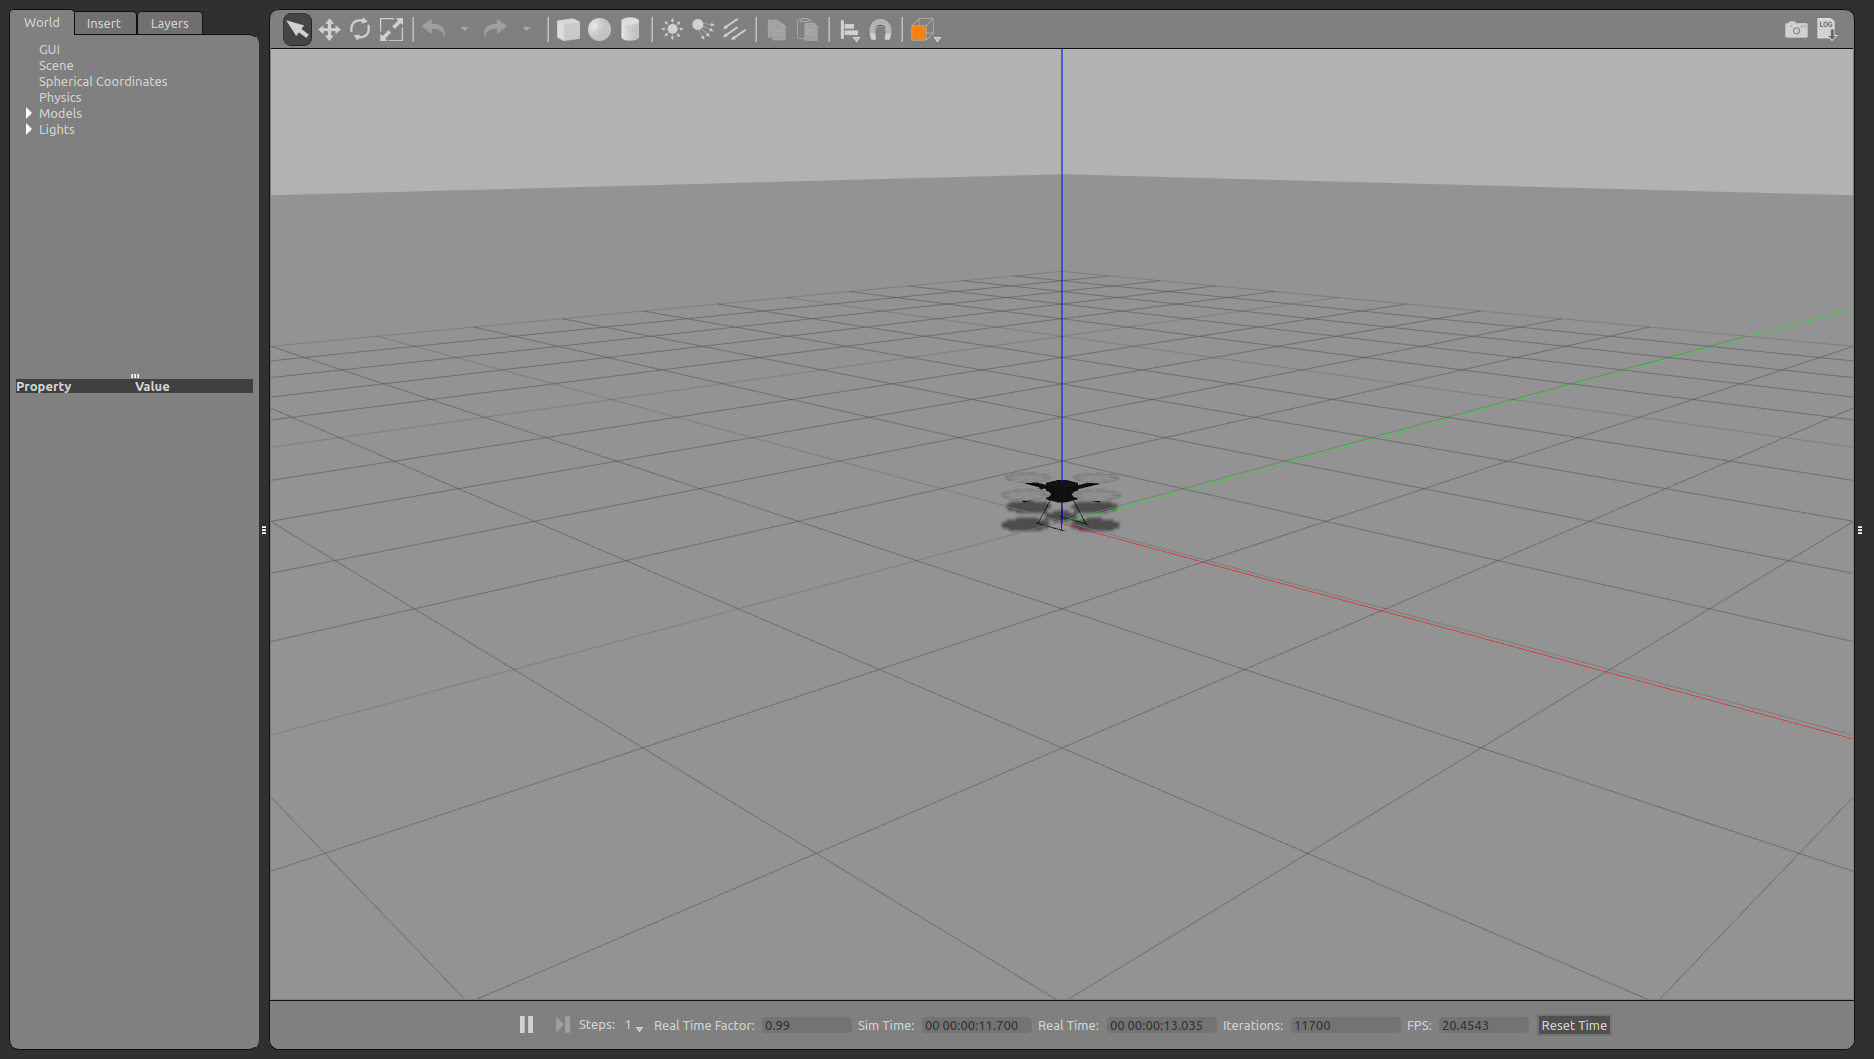
\includegraphics[width=\textwidth]{images/test/drone_gazebo.png}
        \caption{การจำลอง quadrotor ด้วยโปรแกรม Gazebo}
    \end{subfigure}
    \hfill
    \begin{subfigure}[b]{0.8\textwidth}
        \centering
        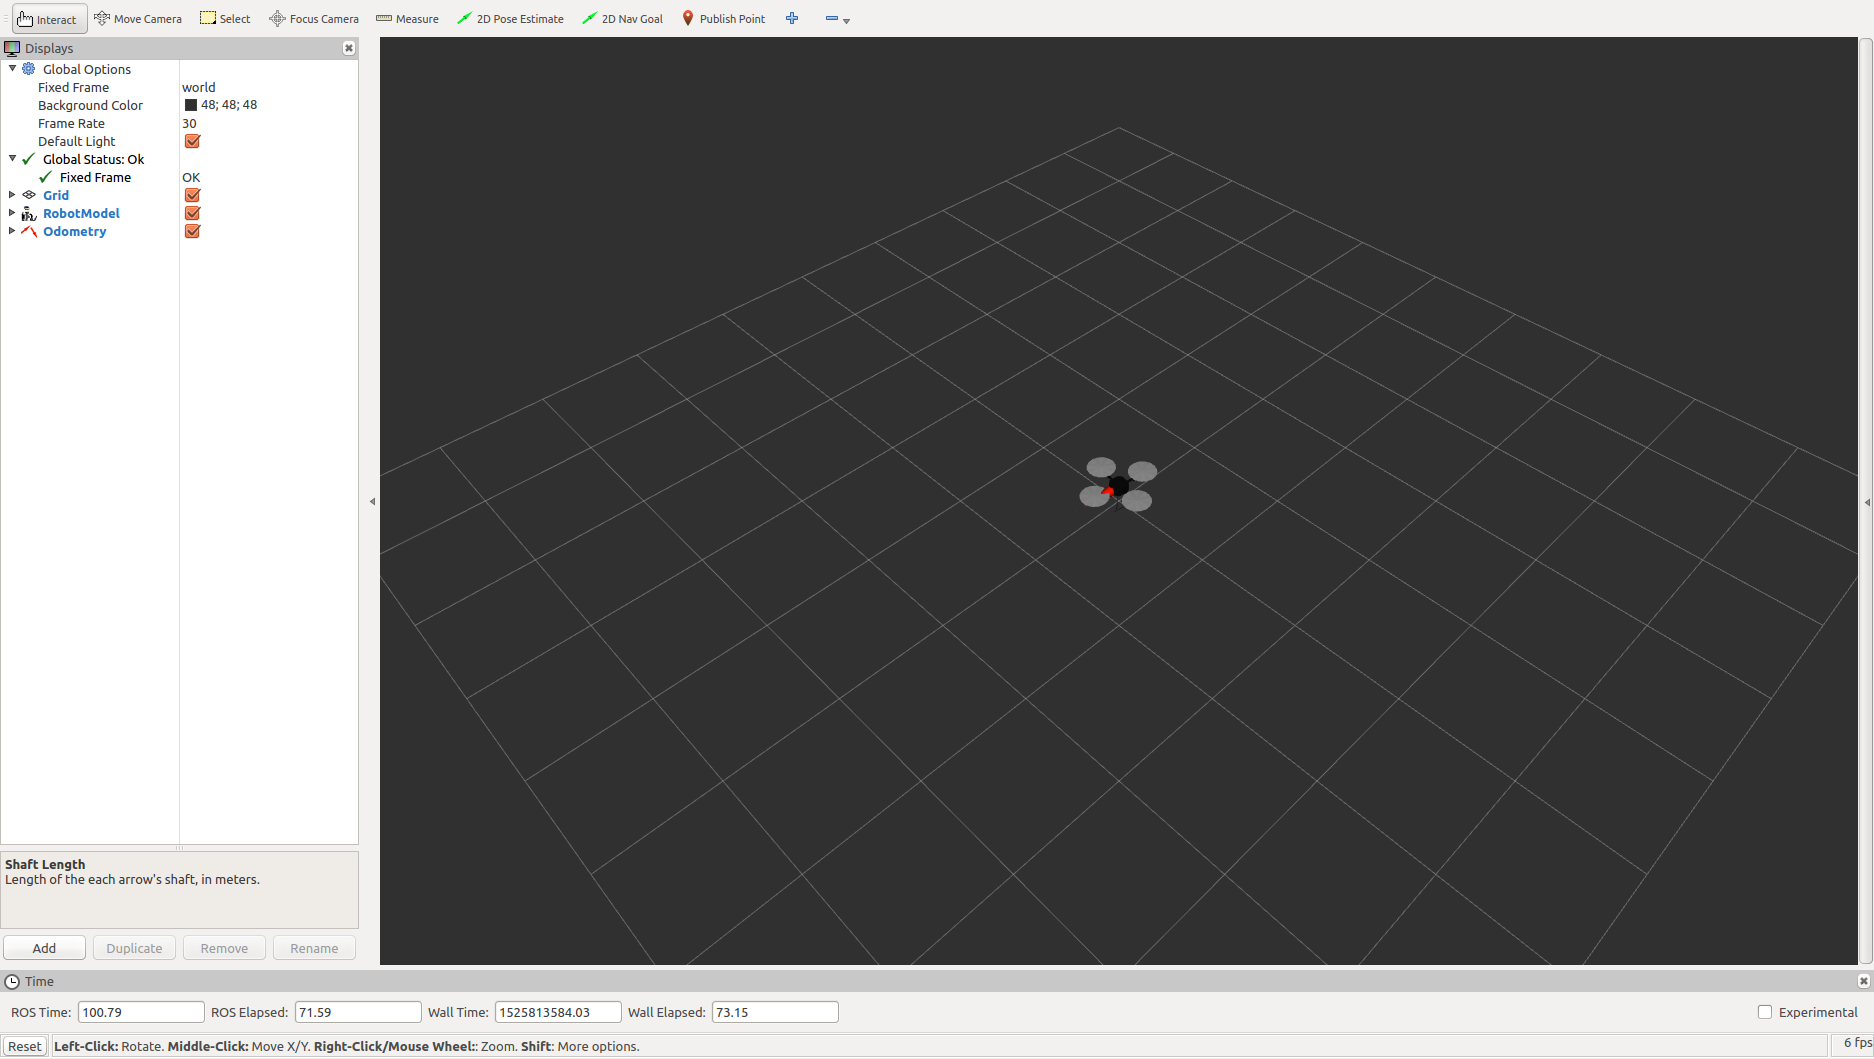
\includegraphics[width=\textwidth]{images/test/drone_rviz.png}
        \caption{การแสดงผลภาพ quadrotor ด้วยโปรแกรม Rviz}
    \end{subfigure}
    \caption{การจำลองและการแสดงผลภาพของ quadrotor }
\end{figure}

\clearpage
\subsection{สั่งให้ quadrotor บินขึ้นเหนือพื้น}
\begin{figure}[!ht]
	\centering
	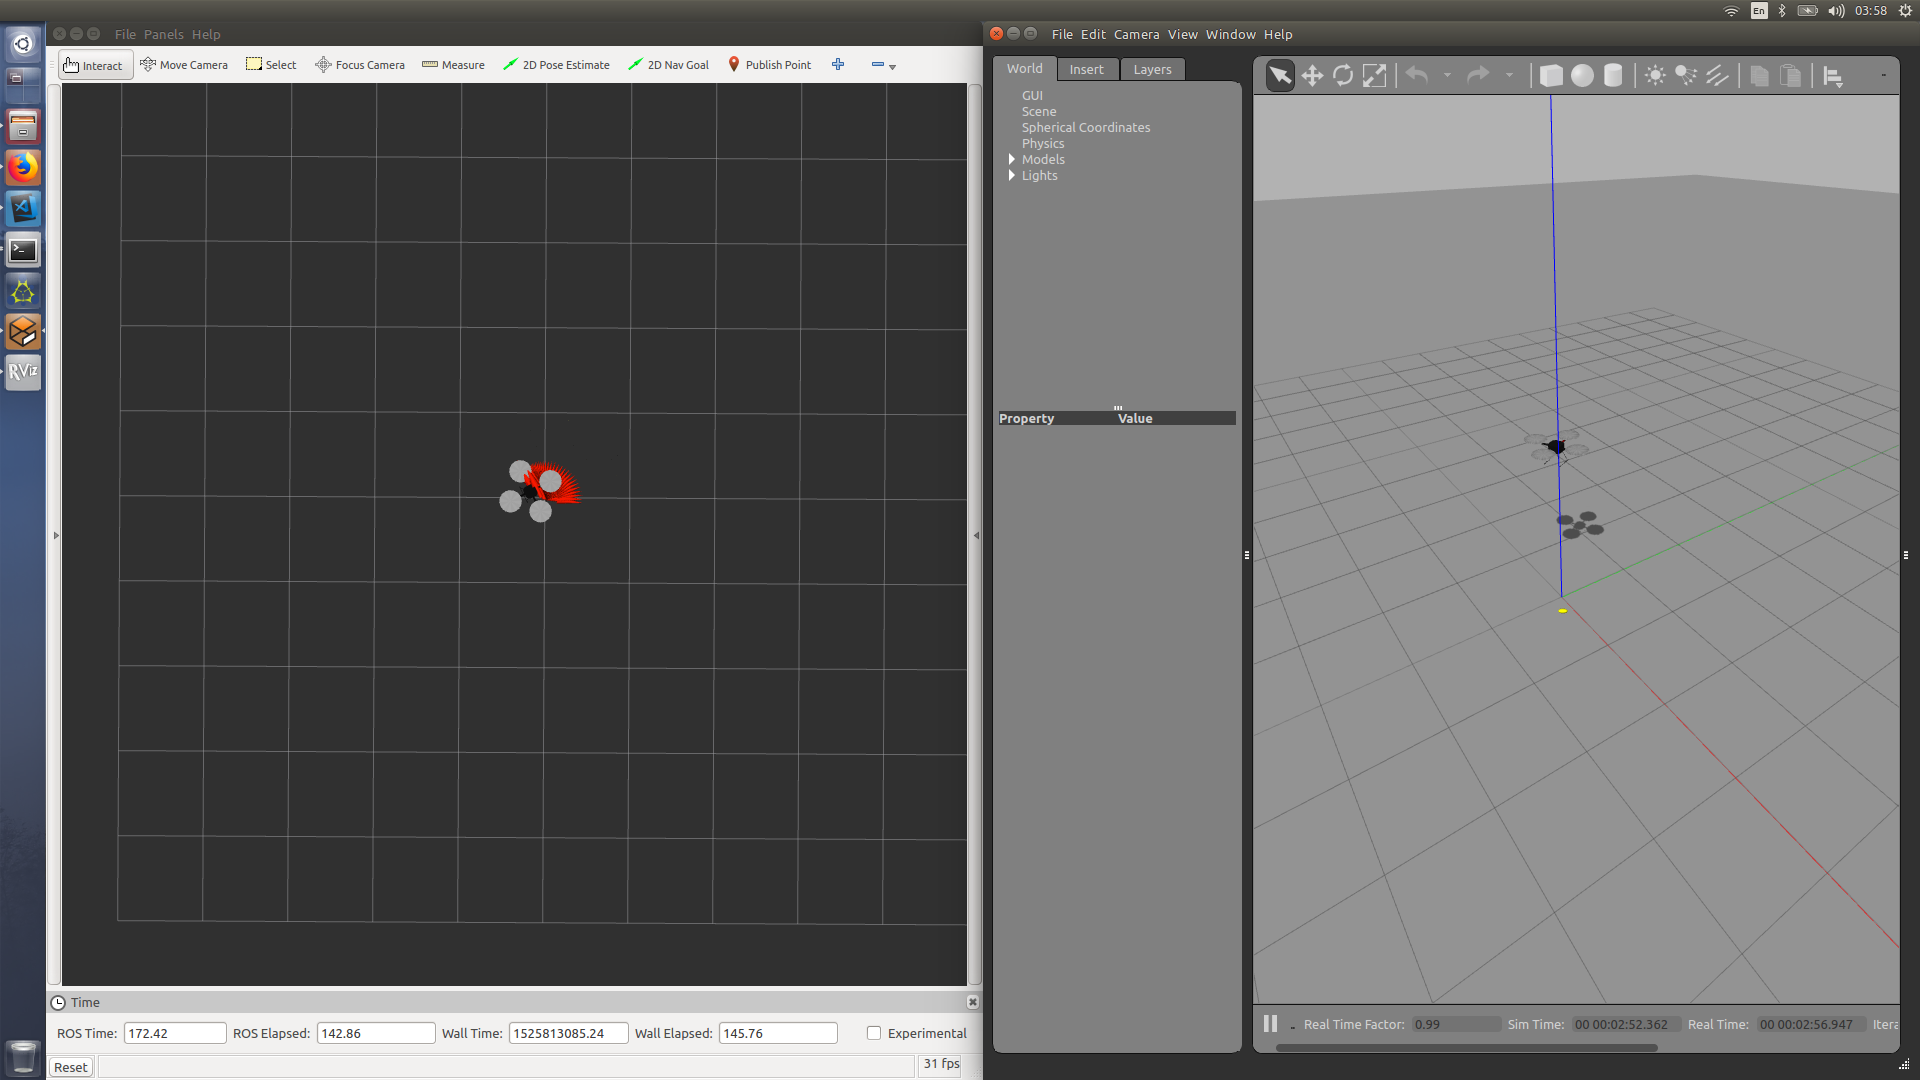
\includegraphics[width=0.7\textwidth]{images/test/drone_takeoff.png}
	\caption{ผลการสั่งให้ quadrotor บินขึ้นเหนือพื้น 2 เมตร}
\end{figure}

\subsection{สั่งให้ quadrotor บินวนเป็นเกลียว}
\begin{figure}[!ht]
    \centering
    \begin{subfigure}[b]{0.67\textwidth}
        \centering
        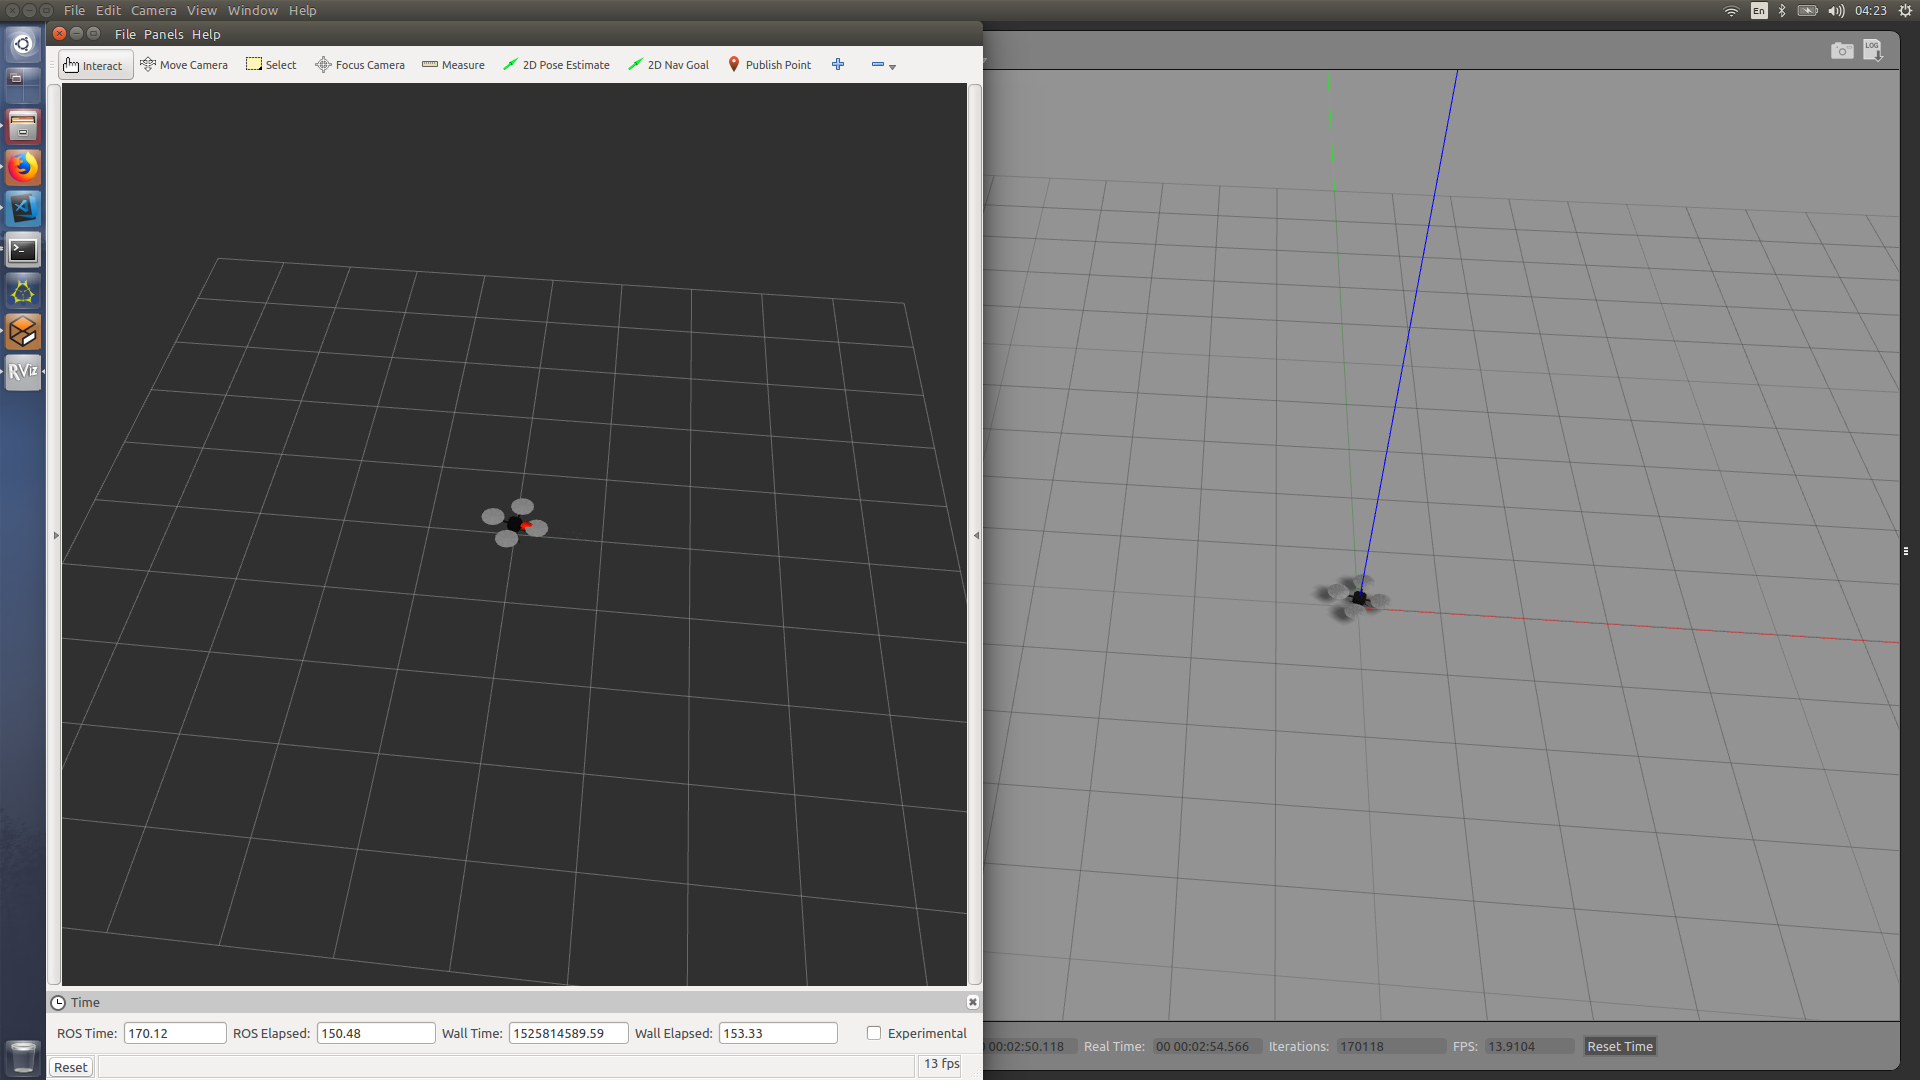
\includegraphics[width=\textwidth]{images/test/circle1.png}
        \caption{quadrotor บินวนเป็นเกลียว ขั้นที่ 1}
    \end{subfigure}
    \hfill
    \begin{subfigure}[b]{0.67\textwidth}
        \centering
        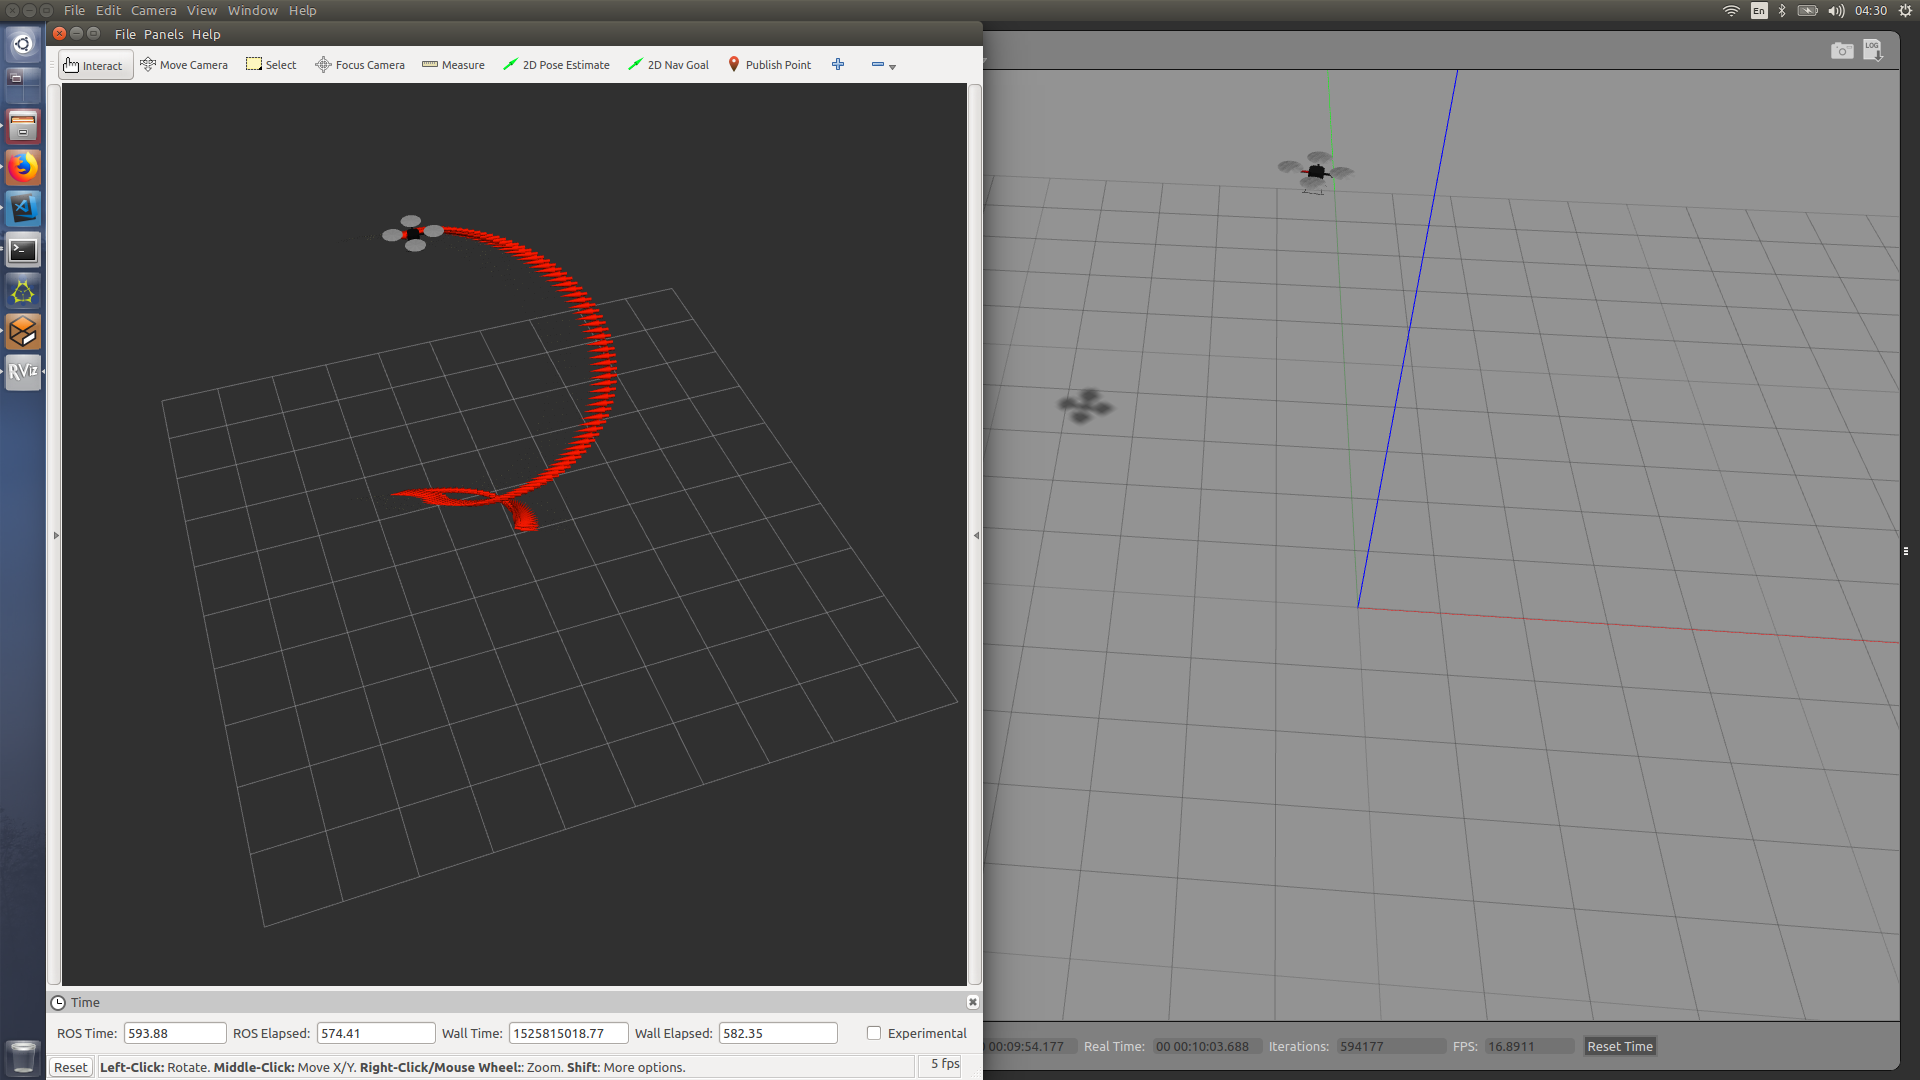
\includegraphics[width=\textwidth]{images/test/circle2.png}
        \caption{quadrotor บินวนเป็นเกลียว ขั้นที่ 2}
    \end{subfigure}
    \caption{ผลการสั่งให้ quadrotor บินวนเป็นเกลียว}
\end{figure}

\clearpage
\subsection{สั่งให้ quadrotor บินเป็นรูปดาว}
\begin{figure}[!ht]
    \centering
    \begin{subfigure}[b]{0.7\textwidth}
        \centering
        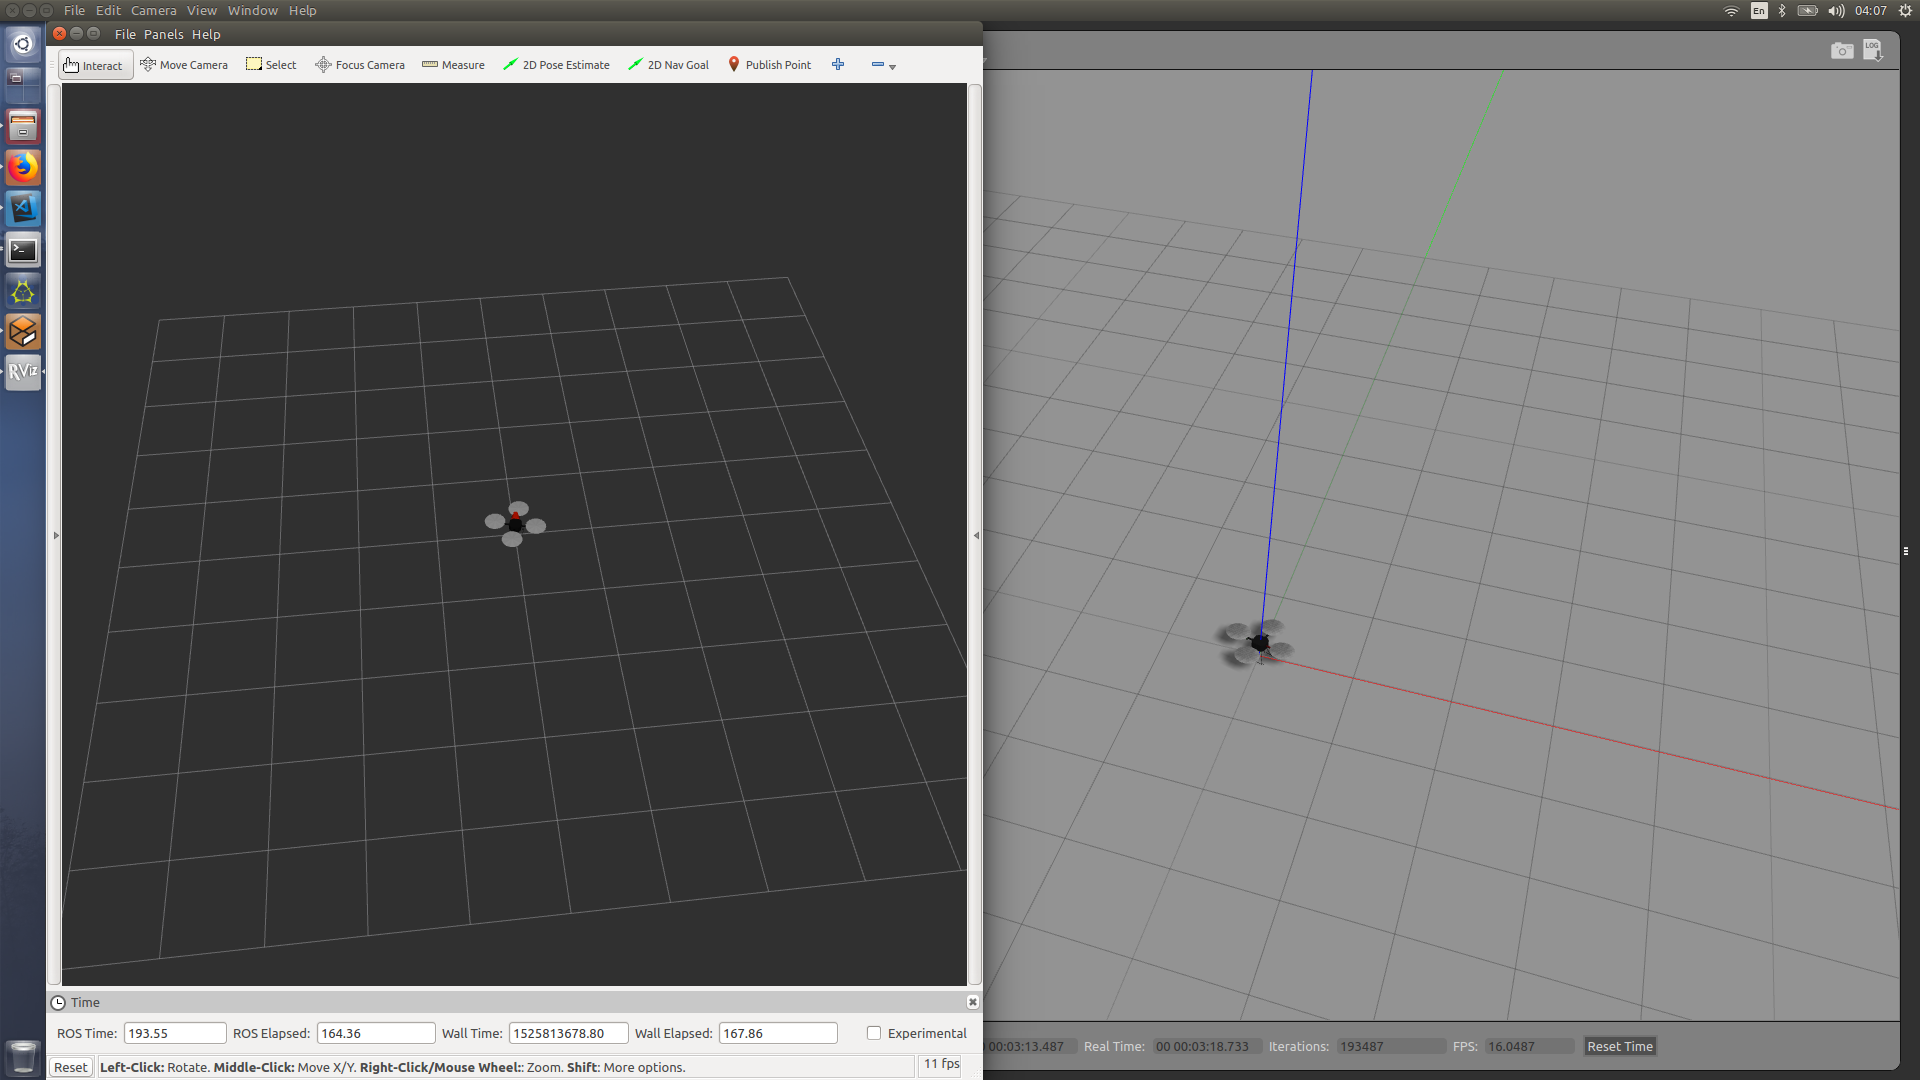
\includegraphics[width=\textwidth]{images/test/drone_rg1.png}
        \caption{quadrotor บินเป็นรูปดาว ขั้นที่ 1}
	\end{subfigure}
	\hfill
    \begin{subfigure}[b]{0.7\textwidth}
        \centering
        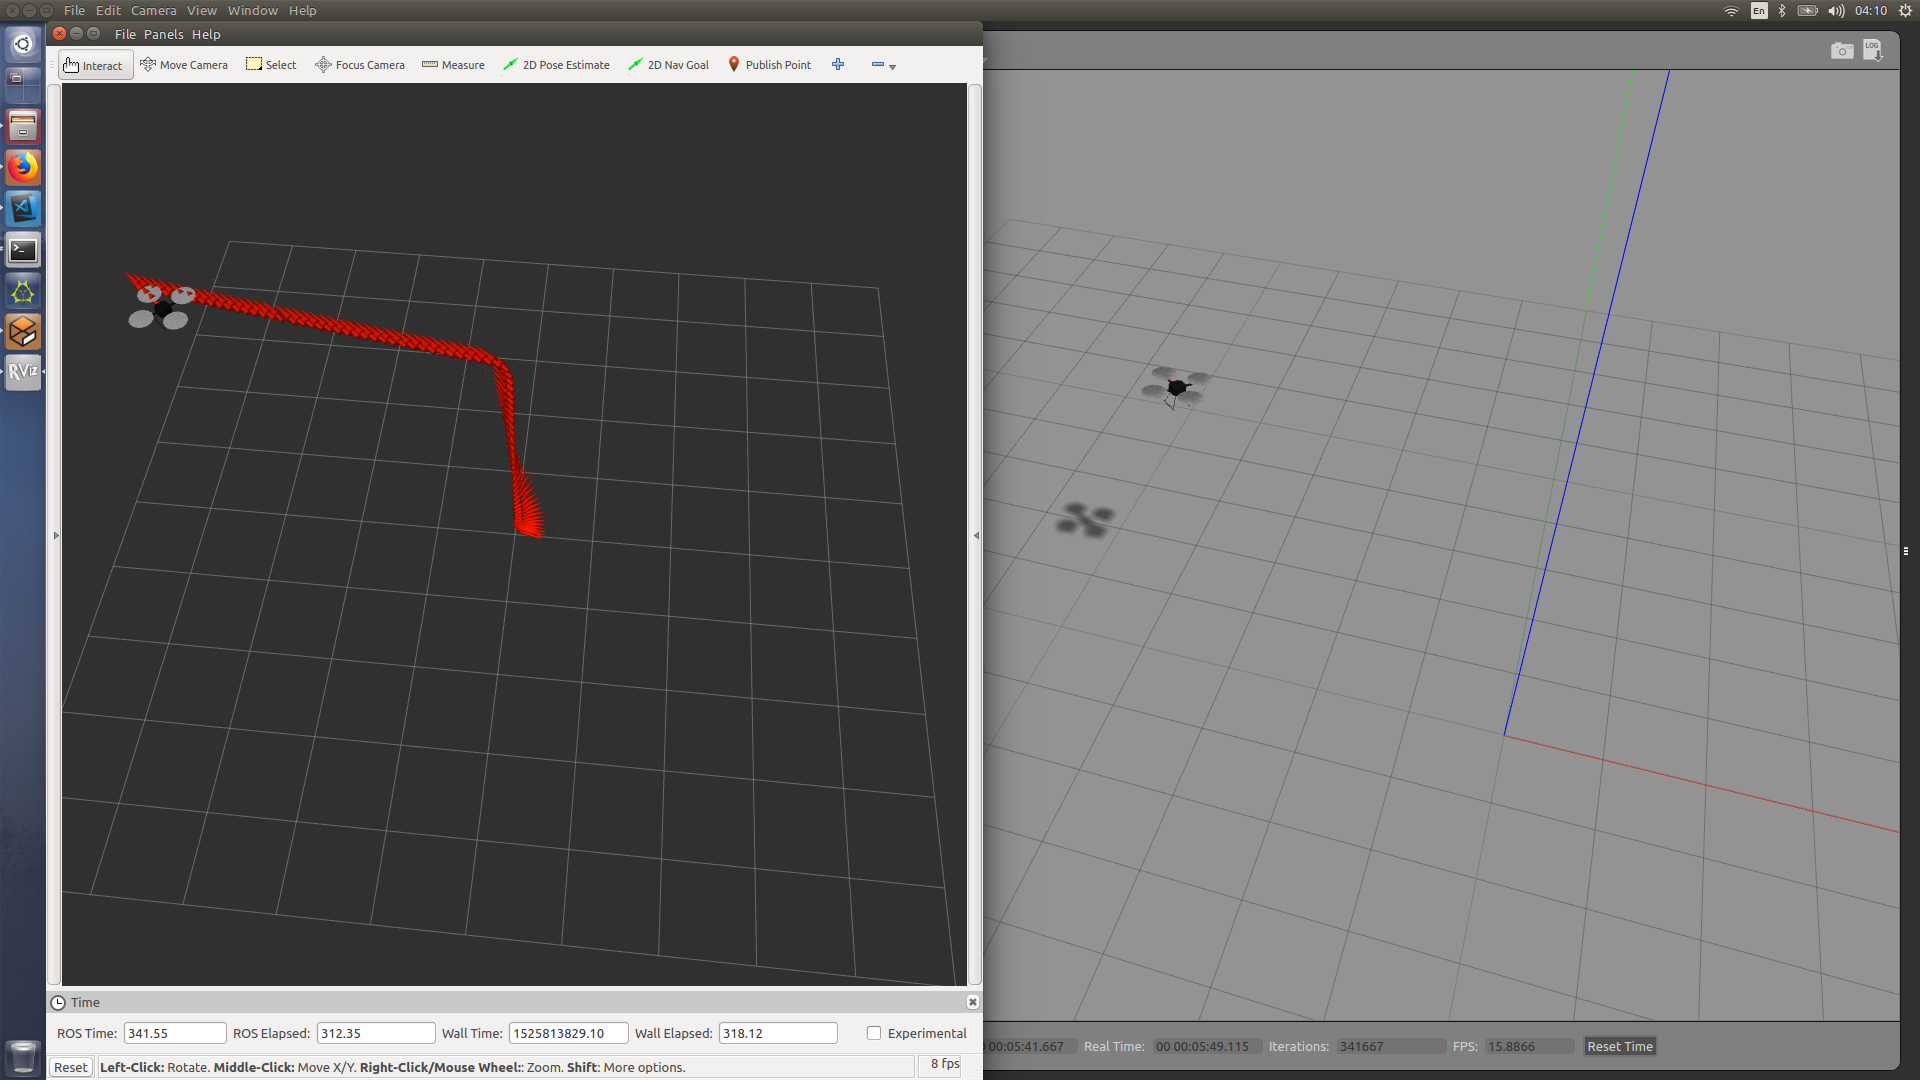
\includegraphics[width=\textwidth]{images/test/drone_rg2.png}
        \caption{quadrotor บินเป็นรูปดาว ขั้นที่ 2}
    \end{subfigure}
    \hfill
    \begin{subfigure}[b]{0.7\textwidth}
        \centering
        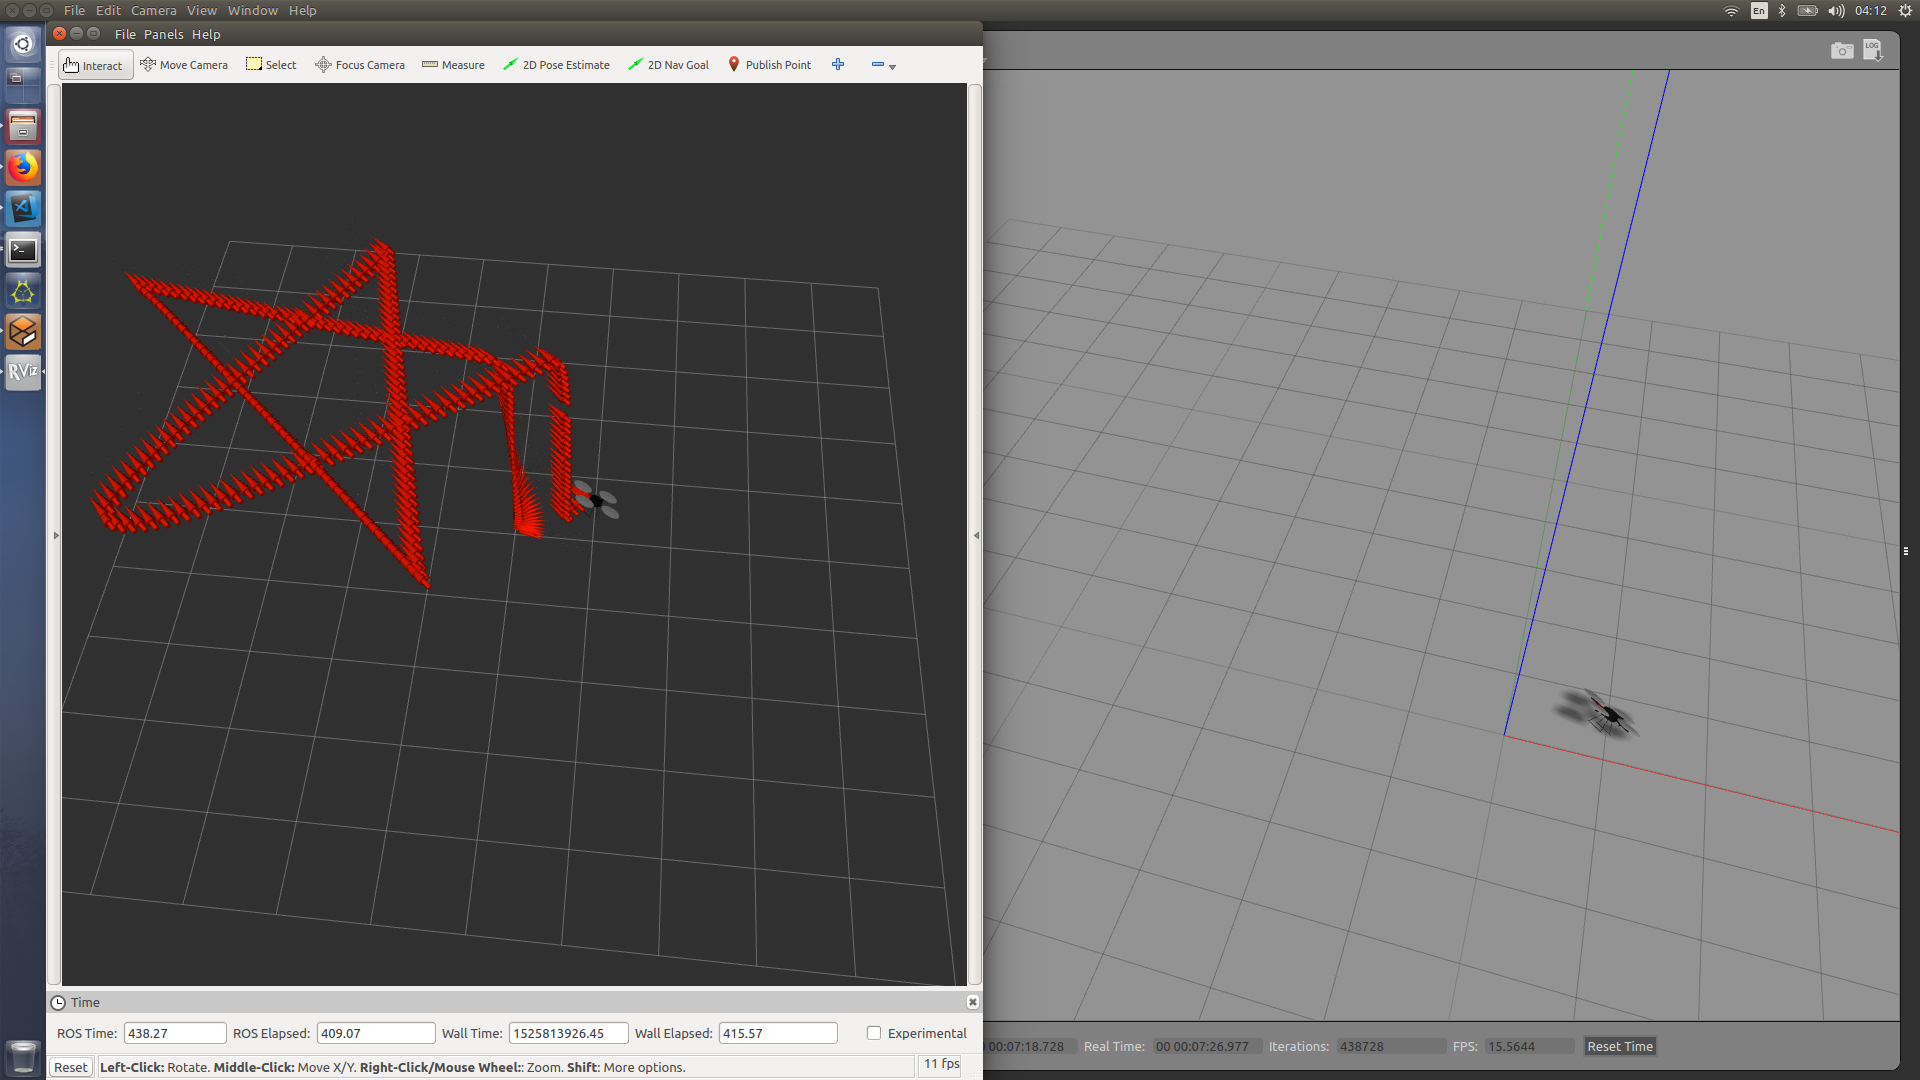
\includegraphics[width=\textwidth]{images/test/drone_rg3.png}
        \caption{quadrotor บินเป็นรูปดาว ขั้นที่ 3}
    \end{subfigure}
    \caption{ผลการสั่งให้ quadrotor บินเป็นรูปดาว}
\end{figure}

\chapter{Analysis/Discussion}
\chapter{Conclusion}


\nocite{*}
\bibliographystyle{plain}
\bibliography{pages/reference}
\addcontentsline{toc}{chapter}{เอกสารอ้างอิง}
\end{document}